% ==============================================================================
% CHƯƠNG 6: KIỂM THỬ VÀ ĐÁNH GIÁ HỆ THỐNG
% ==============================================================================

\chapter{Kiểm thử và đánh giá hệ thống}
\label{chap:kiem-thu-danh-gia}

% Bộ style TikZ đồng bộ toàn báo cáo
\tikzset{
    ragbox/.style={
        rectangle,
        rounded corners=3pt,
        minimum width=2.8cm,
        minimum height=0.85cm,
        text centered,
        align=center,
        draw=primaryBlue,
        line width=0.8pt,
        fill=primaryBlue!8,
        font=\small\sffamily
    },
    ragdb/.style={
        cylinder,
        shape border rotate=90,
        aspect=0.22,
        minimum width=2.4cm,
        minimum height=1.0cm,
        text centered,
        align=center,
        draw=primaryBlue!85!black,
        line width=0.8pt,
        fill=primaryBlue!18,
        font=\small\sffamily
    },
    ragdecision/.style={
        diamond,
        aspect=2.1,
        inner sep=2pt,
        text centered,
        align=center,
        draw=primaryBlue!90!black,
        line width=0.8pt,
        fill=primaryBlue!14,
        font=\small\sffamily
    },
    raggroup/.style={
        rectangle,
        rounded corners=5pt,
        draw=primaryBlue!60,
        dashed,
        line width=0.9pt,
        fill=primaryBlue!3,
        inner sep=8pt
    },
    ragarrow/.style={
        -{Stealth[length=2.4mm, width=1.8mm]},
        line width=0.85pt,
        draw=primaryBlue!85!black
    },
    ragdashed/.style={
        -{Stealth[length=2.2mm, width=1.6mm]},
        line width=0.75pt,
        dashed,
        draw=primaryBlue!70!black
    }
}

\section{Chiến lược và môi trường kiểm thử}
\label{sec:chien-luoc-kiem-thu}

Chương này trình bày bằng chứng thực nghiệm kiểm chứng các yêu cầu chức năng (Mục~\ref{sec:dac-ta-chuc-nang}) và yêu cầu phi chức năng (Mục~\ref{subsec:hieu-nang}) đã đặc tả ở Chương~\ref{chap:phan-tich-yeu-cau}. Mỗi mục gắn với một lớp bằng chứng cụ thể, và toàn bộ số liệu định lượng đều truy xuất được từ các tệp kết quả thô trong thư mục \texttt{backend\_\allowbreak{}rag/\allowbreak{}benchmark/\allowbreak{}results}.

Hệ thống được kiểm thử theo bốn lớp bằng chứng, sắp xếp tăng dần theo mức độ tiệm cận hành vi người dùng thực tế. Bảng~\ref{tab:bon-lop-kiem-thu} tổng hợp công cụ, đối tượng và câu hỏi kiểm chứng của từng lớp.

\begin{table}[htbp]
\centering
\caption{Bốn lớp bằng chứng kiểm thử và mục đích của từng lớp}
\label{tab:bon-lop-kiem-thu}
\small
\begin{tabularx}{\textwidth}{
  >{\raggedright\arraybackslash}p{3.0cm}
  >{\raggedright\arraybackslash}p{3.0cm}
  >{\raggedright\arraybackslash}p{4.3cm}
  >{\raggedright\arraybackslash}X
}
\toprule
\textbf{Lớp} & \textbf{Công cụ} & \textbf{Đối tượng kiểm thử} & \textbf{Câu hỏi cần trả lời} \\
\midrule
Đơn vị và thành phần & Jest~30.x, Vitest~2.x & Hàm thuần, \texttt{guard}, \texttt{DTO}, cổng kiểm soát chất lượng, cơ chế đồng bộ & Từng quy tắc nghiệp vụ có vận hành đúng thiết kế không \\
\midrule
Tích hợp & Jest với cơ sở dữ liệu trong bộ nhớ & Controller, service, lược đồ Mongoose, tương tác truy vấn & Các thành phần khi ghép nối có bảo toàn bất biến và quyền sở hữu dữ liệu không \\
\midrule
Đầu cuối (E2E) & Jest cấu hình E2E riêng, Playwright~1.x & Hợp đồng HTTP đầy đủ, giao diện trên trình duyệt thật & Người dùng có hoàn thành trọn vẹn các hành trình chính không \\
\midrule
Đánh giá chất lượng và tải & DeepEval, bộ đo tải k6 & Chất lượng truy hồi, chất lượng sinh văn bản, độ trễ dưới tải & Hệ thống có đạt các ngưỡng định lượng công bố ở Chương~\ref{chap:phan-tich-yeu-cau} không \\
\bottomrule
\end{tabularx}
\end{table}

Hình~\ref{fig:bon-lop-kiem-thu} minh hoạ bốn lớp bằng chứng và mối quan hệ tiến triển giữa chúng trong quy trình đánh giá.

\begin{figure}[htbp]
\centering
\resizebox{\textwidth}{!}{%
\begin{tikzpicture}[
    node distance=0.95cm,
    layernode/.style={ragbox, text width=4.4cm, minimum height=1.8cm, font=\footnotesize\sffamily}
]
    \node[layernode] (l1) {\textbf{Lớp 1: Đơn vị \& Thành phần}\\Hàm thuần, \texttt{guard}, \texttt{DTO}\\Hai cổng kiểm soát chất lượng};
    \node[layernode, right=of l1] (l2) {\textbf{Lớp 2: Tích hợp}\\MongoDB replica set bộ nhớ\\Quyền sở hữu \& xoá mềm};
    \node[layernode, right=of l2] (l3) {\textbf{Lớp 3: Đầu cuối (E2E)}\\Hợp đồng HTTP đầy đủ\\Trình duyệt thật Playwright};
    \node[layernode, right=of l3] (l4) {\textbf{Lớp 4: Chất lượng \& Tải}\\DeepEval trên bộ 150~câu\\Bộ đo tải k6 bốn tầng};

    \draw[ragarrow] (l1) -- (l2);
    \draw[ragarrow] (l2) -- (l3);
    \draw[ragarrow] (l3) -- (l4);
\end{tikzpicture}%
}
\caption{Bốn lớp bằng chứng kiểm thử và mối quan hệ tiến triển giữa chúng}
\label{fig:bon-lop-kiem-thu}
\end{figure}

Môi trường kiểm thử được cấu hình phản ánh đúng điều kiện vận hành thực tế thay vì tối ưu hoá giả tạo cho kịch bản đo. Năm yếu tố môi trường chi phối trực tiếp độ tin cậy của toàn bộ số liệu đo được:

\begin{itemize}
\item[--] \textbf{Chất lượng dữ liệu kiểm thử}: Bộ đánh giá truy hồi gồm 150~câu hỏi khoa học (100~câu có đáp án trong kho và 50~câu ngoài phạm vi); cơ sở dữ liệu kiểm thử tải được nạp sẵn 1.500~phiên trò chuyện và 15.000~tin nhắn kèm trích dẫn, tạo kích thước phản hồi trung bình khoảng 4,6~KB thay vì đo trên bảng rỗng.
\item[--] \textbf{Độ trễ mạng thực qua \texttt{tunnel}}: Cơ sở dữ liệu ứng dụng trong đợt đo tải nằm sau \texttt{tunnel} Cloudflare Access với độ trễ khứ hồi (\texttt{RTT}) thực đo là 114~ms (cao hơn đáng kể so với mức 15--25~ms ở cấu hình phát triển tối ưu nêu tại Chương~\ref{chap:dong-goi-van-hanh}); mọi phép đo đầu cuối và ghi dữ liệu đều gánh trực tiếp chi phí khứ hồi này.
\item[--] \textbf{Tính lặp lại của phép đo tải}: Mỗi đợt đo lặp lại trên cùng tập dữ liệu và cùng phân bố lưu lượng để bảo đảm độ trễ và tỉ lệ lỗi giữa các cấu hình trước và sau tối ưu có thể so sánh trực tiếp.
\item[--] \textbf{Tách biệt bộ phát tải và tiến trình phục vụ}: Công cụ k6 chạy ngoài tiến trình máy chủ ứng dụng, còn mô hình nhúng và mô hình sinh văn bản chạy trong tiến trình máy chủ trên phần cứng GPU chuyên biệt (NVIDIA RTX~4060, 8~GB VRAM, CUDA); do đó phép đo phản ánh đầy đủ cả chi phí truyền nhận qua giao diện lập trình ứng dụng.
\item[--] \textbf{Kiểm chứng nội dung phản hồi (\texttt{checks})}: Mọi phản hồi trong kịch bản đo tải đều được kiểm tra cấu trúc dữ liệu bắt buộc chứ không chỉ dựa vào mã trạng thái HTTP; một phản hồi trả về HTTP~200 nhưng thiếu trường dữ liệu vẫn bị tính là khẳng định thất bại.
\end{itemize}

Hai quy ước báo cáo được áp dụng thống nhất xuyên suốt chương. Thứ nhất, mọi kịch bản đo thông lượng ứng dụng đều sử dụng mô hình tải mở (\texttt{ramping-\allowbreak{}arrival-\allowbreak{}rate}) để tần suất yêu cầu đến độc lập với tốc độ phản hồi của máy chủ, qua đó loại bỏ sai lệch do hiện tượng \texttt{coordinated omission} (trong mô hình tải đóng, khi máy chủ chậm đi, người dùng ảo tự động giảm nhịp gửi yêu cầu kế tiếp và làm đẹp giả tạo phân vị độ trễ). Thứ hai, tiêu chuẩn chứng nhận tuân theo Quy tắc~L1 đặc tả tại Mục~\ref{subsec:hieu-nang} (Chương~\ref{chap:phan-tich-yeu-cau}): duy trì liên tục 180~giây với độ trễ phân vị 95 (\texttt{p95}) dưới 500~ms, phân vị 99 (\texttt{p99}) dưới 1.000~ms và tỉ lệ lỗi dưới 1\%. Kết quả chứng nhận ba tầng tổng hợp ở Mục~\ref{subsec:ket-qua-hieu-nang} (Chương~\ref{chap:ket-luan}, gồm Tầng~A xác định điểm gãy, Tầng~B giữ tải chứng nhận 3~phút và Tầng~C cô lập tải mật mã) được trích xuất trực tiếp từ bộ đo bốn tầng chi tiết trong Mục~\ref{sec:danh-gia-hieu-nang} của chương này.

Một ranh giới phạm vi cần xác lập ngay từ đầu: ba ngưỡng trên chỉ áp dụng cho các đường đọc và thao tác nghiệp vụ không sinh văn bản. Kịch bản hỏi đáp có sinh văn bản được đo tách biệt tại Mục~\ref{sec:danh-gia-rag} và Mục~\ref{subsec:tang-4-llm-queue} do thời gian thực thi bị chi phối bởi năng lực tính toán của mô hình ngôn ngữ lớn chứ không phải tầng truy xuất.

\section{Kiểm thử đơn vị}
\label{sec:unit-testing}

Khối lượng kiểm thử đơn vị và thành phần của toàn hệ thống được tổng hợp tại Bảng~\ref{tab:khoi-luong-unit-test}.

\begin{table}[htbp]
\centering
\caption{Khối lượng kiểm thử đơn vị và thành phần theo phân hệ}
\label{tab:khoi-luong-unit-test}
\small
\begin{tabularx}{\textwidth}{
  >{\raggedright\arraybackslash}p{4.0cm}
  >{\raggedright\arraybackslash}X
  >{\raggedleft\arraybackslash}p{4.2cm}
}
\toprule
\textbf{Phân hệ} & \textbf{Phạm vi} & \textbf{Khối lượng} \\
\midrule
Máy chủ (\texttt{backend\_rag}) & Các mô đun nghiệp vụ, truy xuất và một tệp cấu hình khởi động & 267 khối kiểm thử trong 25 tệp \\
\midrule
Người dùng (\texttt{frontend\_rag}) & Thành phần giao diện, trạng thái và mô phỏng \texttt{IndexedDB} & 327 khối kiểm thử trong 37 tệp \\
\midrule
\textbf{Tổng đơn vị và thành phần} & & \textbf{594 khối kiểm thử trong 62 tệp} \\
\bottomrule
\end{tabularx}
\end{table}

Bảng~\ref{tab:khoi-luong-unit-test} cho thấy độ phủ kiểm thử đơn vị trải đều trên cả hai phân hệ backend và frontend. Ở phía máy chủ, ba nhóm được kiểm thử dày đặc nhất gồm phân hệ quản trị (30~khối), phân hệ quản lý phiên trò chuyện (26~khối) và phân hệ hỏi đáp RAG (22~khối, trong đó có 11~khối kiểm chứng riêng cho hai cổng kiểm soát chất lượng). Ba quyết định thiết kế sau quyết định trực tiếp độ tin cậy của bộ kiểm thử đơn vị:

\begin{itemize}
\item[--] \textbf{Thay thế mô hình AI thật bằng bộ giả lập tất định}: Hai cổng kiểm soát chất lượng trước và sau sinh được kiểm thử bằng bộ giả lập thay cho mô hình ngôn ngữ thật, giúp xác minh chính xác các ngưỡng cắt, nhánh viết lại câu hỏi, thời hạn chờ và nhánh từ chối mà không phụ thuộc GPU.
\item[--] \textbf{Kiểm thử chính sách biên trực tiếp tại \texttt{guard} và \texttt{decorator}}: Quy tắc xác thực, phân quyền vai trò và giới hạn tần suất được kiểm chứng trực tiếp ở mức \texttt{guard} để phát hiện sớm sai lệch bảo mật mà không cần dựng toàn bộ ngăn xếp HTTP.
\item[--] \textbf{Cô lập kho cục bộ trình duyệt phía frontend}: Toàn bộ 327~khối kiểm thử giao diện vận hành trên bộ giả lập \texttt{IndexedDB}, giúp kiểm chứng logic đồng bộ ngoại tuyến và khôi phục phiên trò chuyện hoàn toàn độc lập với máy chủ backend.
\end{itemize}

Đoạn trích dưới đây trong \texttt{rag.gates.spec.ts} (thuộc thư mục \texttt{backend\_\allowbreak{}rag/\allowbreak{}src/\allowbreak{}modules/\allowbreak{}rag/}) minh hoạ cách kiểm thử tất định hai cổng kiểm soát chất lượng làm cơ sở cho các đánh giá định lượng ở Mục~\ref{sec:danh-gia-retrieval} và Mục~\ref{sec:danh-gia-rag}:

\begin{tsbox}{Kiểm thử tất định hai cổng kiểm soát chất lượng trong rag.gates.spec.ts}
it('enough evidence: reranks, answers and reports the scores', async () => {
  const result = await run(setup({ relevance: [[0.9]] }));
  expect(result.quality?.evidence_score).toBe(0.9);
  expect(result.quality?.abstained).toBe(false);
  expect(result.answer).toContain('[Paper: a]');
});
\end{tsbox}

\section{Kiểm thử tích hợp}
\label{sec:integration-testing}

Kiểm thử tích hợp xác minh hành vi phối hợp giữa tầng controller, service, lược đồ Mongoose và lớp truy vấn trên một cụm MongoDB replica set chạy thật trong bộ nhớ. Phân hệ quản lý phiên trò chuyện có độ phủ cao nhất với 34~kịch bản có mã định danh cố định, trong đó Bảng~\ref{tab:kich-ban-tich-hop-session} phân loại 30~kịch bản cốt lõi theo sáu nhóm bất biến (4~kịch bản còn lại kiểm tra các trường hợp biên của vỏ bọc phản hồi và siêu dữ liệu phân trang).

\begin{table}[htbp]
\centering
\caption{Cấu trúc kịch bản tích hợp cốt lõi của phân hệ quản lý phiên trò chuyện}
\label{tab:kich-ban-tich-hop-session}
\small
\begin{tabularx}{\textwidth}{
  >{\raggedright\arraybackslash}p{4.4cm}
  >{\raggedleft\arraybackslash}p{1.9cm}
  >{\raggedright\arraybackslash}X
}
\toprule
\textbf{Nhóm kịch bản} & \textbf{Số lượng} & \textbf{Nội dung kiểm chứng} \\
\midrule
Quy tắc hàm thuần & 5 & Chuẩn hoá tiêu đề, giới hạn 120 ký tự Unicode, định dạng mốc thời gian UTC cộng dồn \\
\midrule
Xác thực và quyền sở hữu & 6 & Từ chối thiếu token, trả mã 404 khi đọc hoặc ghi vào phiên thuộc tài khoản khác \\
\midrule
Vòng đời phân trang con trỏ & 5 & Kích thước trang cố định, cô lập dữ liệu theo chủ sở hữu, phân trang không trùng lặp và từ chối con trỏ giả mạo \\
\midrule
Tìm kiếm và chống tiêm mã & 4 & Tìm kiếm không phân biệt hoa thường, thoát ký tự đặc biệt regex, chặn truy vấn đối tượng NoSQL và kháng \texttt{ReDoS} \\
\midrule
Ranh giới và vòng đời tin nhắn & 6 & Giới hạn 200 tin nhắn mỗi phiên, từ chối tham số vượt độ dài, xoá mềm hai tầng và xác nhận trạng thái xoá mềm \\
\midrule
Khởi tạo và ghi dữ liệu & 4 & Tạo lặp \texttt{idempotent}, định danh \texttt{UUIDv7}, bảo toàn thứ tự tin nhắn và hỗ trợ ghi tuần tự khi thiếu transaction \\
\bottomrule
\end{tabularx}
\end{table}

Bảng~\ref{tab:kich-ban-tich-hop-session} cho thấy trọng tâm của kiểm thử tích hợp nằm ở tính toàn vẹn bất biến dữ liệu hơn là đo thông lượng đọc thuần tuý. Ba quyết định cài đặt dưới đây tạo nên giá trị bảo chứng của bộ kiểm thử tích hợp:

\begin{itemize}
\item[--] \textbf{Kiểm chứng trên cụm replica set thật}: Các thao tác ghi phiên kèm tin nhắn được kiểm thử trên cụm replica set thật trong bộ nhớ để xác nhận tính nguyên tử của transaction đa tài liệu.
\item[--] \textbf{Kiểm thử cơ chế dự phòng không có transaction}: Một nhóm kịch bản riêng thực thi trên nút MongoDB đơn lẻ để chứng minh luồng ghi tuần tự vẫn vận hành an toàn khi môi trường không hỗ trợ transaction.
\item[--] \textbf{Kiểm thử chống tiêm mã ngay ở lớp truy vấn}: Các tải trọng NoSQL injection và chuỗi regex gây treo (\texttt{ReDoS}) được đưa qua toàn bộ lớp \texttt{DTO} và câu truy vấn Mongoose thực tế thay vì chỉ kiểm tra hàm tiện ích đơn lẻ.
\end{itemize}

\section{Kiểm thử đầu cuối}
\label{sec:e2e-testing}

Bảng~\ref{tab:khoi-luong-e2e} tổng hợp khối lượng kiểm thử đầu cuối trên cả hai phân hệ máy chủ và giao diện trình duyệt.

\begin{table}[htbp]
\centering
\caption{Khối lượng kiểm thử đầu cuối trên hai phân hệ của hệ thống}
\label{tab:khoi-luong-e2e}
\small
\begin{tabularx}{\textwidth}{
  >{\raggedright\arraybackslash}p{3.4cm}
  >{\raggedright\arraybackslash}p{3.4cm}
  >{\raggedright\arraybackslash}X
  >{\raggedleft\arraybackslash}p{2.3cm}
}
\toprule
\textbf{Phân hệ} & \textbf{Công cụ} & \textbf{Phạm vi} & \textbf{Khối lượng} \\
\midrule
Máy chủ (\texttt{backend\_rag}) & Jest~30.x (cấu hình E2E riêng) & Đăng ký, đăng nhập, hỏi đáp RAG, quản lý phiên trò chuyện, hợp đồng HTTP & 13 kịch bản \\
\midrule
Người dùng (\texttt{frontend\_rag}) & Playwright~1.x trên trình duyệt thật & Hành trình cây tri thức 3D, hồi quy hình ảnh, luồng xác thực & 26 kịch bản \\
\bottomrule
\end{tabularx}
\end{table}

Kịch bản đầu cuối tiêu biểu ở phía máy chủ kiểm chứng chuỗi nghiệp vụ khép kín qua API thật: đăng ký tài khoản, đăng nhập, gửi câu hỏi RAG, truy xuất danh sách và chi tiết phiên trò chuyện, đọc chi tiết bài báo theo lô, xoay vòng refresh token, thử tái sử dụng token cũ để kích hoạt thu hồi họ token, và đăng xuất. Toàn bộ kịch bản chạy trên máy chủ NestJS thật kết nối cơ sở dữ liệu thật nhằm xác thực hợp đồng HTTP liên hoàn thay vì các điểm gọi rời rạc.

Ở phía giao diện, 26~kịch bản Playwright chia thành ba vai trò: 7~kịch bản xác minh tương tác điều hướng và chọn nút trên không gian tri thức ba chiều; 17~kịch bản hồi quy hình ảnh đối chiếu ảnh chụp màn hình nhằm phát hiện sai lệch bố cục hoặc kết xuất WebGL; và 2~kịch bản xác thực kiểm chứng thanh trạng thái khi chưa đăng nhập cũng như mở khoá khung soạn thảo khi có phiên lưu cục bộ.

Số lượng kịch bản đầu cuối phía người dùng gấp đôi phía máy chủ do mục tiêu kiểm định khác biệt: phía máy chủ tập trung kiểm chứng tính đúng đắn của hợp đồng API và bất biến bảo mật, còn phía người dùng cần bao phủ đồng thời tương tác đồ hoạ 3D, tính ổn định hiển thị và trạng thái lưu trữ ngoại tuyến trên trình duyệt thật.

\section{Kiểm thử chức năng và nghiệp vụ}
\label{sec:kiem-thu-chuc-nang}

Để đối chiếu có hệ thống năm nhóm yêu cầu chức năng (Mục~\ref{subsec:quan-ly-nguoi-dung}--\ref{subsec:quan-ly-lich-su}) và năm trường hợp sử dụng (\texttt{UC-1}--\texttt{UC-5}) đã đặc tả ở Chương~\ref{chap:phan-tich-yeu-cau}, Chương~6 phân rã các yêu cầu nghiệp vụ cốt lõi thành chín mã đối chiếu \texttt{FR-01}--\texttt{FR-09} kèm bằng chứng kiểm thử tương ứng tại Bảng~\ref{tab:doi-chieu-chuc-nang}.

\begin{table}[htbp]
\centering
\caption{Đối chiếu chín nhóm yêu cầu chức năng từ Chương~2 với bằng chứng kiểm thử}
\label{tab:doi-chieu-chuc-nang}
\small
\begin{tabularx}{\textwidth}{
  >{\raggedright\arraybackslash}p{1.6cm}
  >{\raggedright\arraybackslash}p{4.5cm}
  >{\raggedright\arraybackslash}X
  >{\raggedright\arraybackslash}p{1.6cm}
}
\toprule
\textbf{Mã} & \textbf{Nhóm yêu cầu (Chương~2)} & \textbf{Bằng chứng kiểm thử} & \textbf{Kết quả} \\
\midrule
\texttt{FR-01} & Đăng ký, đăng nhập, làm mới, thu hồi token và quản lý hồ sơ (Mục~\ref{subsec:quan-ly-nguoi-dung}, \texttt{UC-1}) & 26 khối kiểm thử đơn vị phân hệ xác thực và 8 khối kiểm thử danh sách mật khẩu bị cấm & Đạt \\
\midrule
\texttt{FR-02} & Tìm kiếm ngữ nghĩa và đọc bài báo theo lô tối đa 20 bài (Mục~\ref{subsec:tim-kiem-paper}, \texttt{UC-3}) & Kịch bản E2E đọc hàng loạt bài báo, kiểm tra mã lỗi khi thiếu bài; kiểm thử đơn vị kho khoa học & Đạt \\
\midrule
\texttt{FR-03} & Hỏi đáp có trích dẫn và truyền phát sự kiện \texttt{SSE} (Mục~\ref{subsec:tuong-tac-ai}, \texttt{UC-2}) & Kịch bản E2E hỏi đáp không token trả \texttt{session\_id} rỗng; 11 khối kiểm thử hai cổng chất lượng & Đạt \\
\midrule
\texttt{FR-04} & Tuỳ chỉnh tham số truy hồi: lĩnh vực, \texttt{top\_k}, số nhánh (Mục~\ref{subsec:tuong-tac-ai}) & Kiểm thử biên giá trị và xác thực kiểu dữ liệu trong \texttt{DTO} & Đạt \\
\midrule
\texttt{FR-05} & Quản lý phiên trò chuyện: liệt kê, tìm kiếm, đổi tên, xoá mềm (Mục~\ref{subsec:quan-ly-lich-su}, \texttt{UC-4}) & 34 kịch bản tích hợp có mã định danh của phân hệ quản lý phiên trò chuyện & Đạt \\
\midrule
\texttt{FR-06} & Trực quan hoá cây tri thức ba chiều trên WebGL (Mục~\ref{subsec:tim-kiem-paper}) & 7 kịch bản hành trình cây tri thức và 17 kịch bản hồi quy hình ảnh trên Playwright & Đạt \\
\midrule
\texttt{FR-07} & Lưu trữ cục bộ trình duyệt và đọc lại lịch sử khi ngoại tuyến (Mục~\ref{subsec:quan-ly-lich-su}) & Nhóm kiểm thử đồng bộ và phục hồi ngoại tuyến trên bộ giả lập \texttt{IndexedDB} (\texttt{RagChatDB}) & Đạt \\
\midrule
\texttt{FR-08} & Bảo mật, phân quyền quản trị và giới hạn tần suất (Mục~\ref{subsec:bao-mat}, \texttt{UC-5}) & 30 khối kiểm thử phân hệ quản trị và 10 khối kiểm thử giới hạn tần suất theo nhóm route & Đạt \\
\midrule
\texttt{FR-09} & Suy giảm mềm khi thành phần AI hoặc dữ liệu bổ trợ gián đoạn (Mục~\ref{subsec:do-tin-cay}) & Kiểm thử endpoint kiểm tra sức khoẻ ba trạng thái (\texttt{ok}, \texttt{degraded}, \texttt{down}) & Đạt \\
\bottomrule
\end{tabularx}
\end{table}

Bảng~\ref{tab:doi-chieu-chuc-nang} xác nhận toàn bộ chín nhóm yêu cầu chức năng đều có bằng chứng kiểm thử trực tiếp. Đáng chú ý là yêu cầu lõi \texttt{FR-03} được bảo chứng độc lập ở cả hai tầng: kiểm thử đơn vị xác minh ranh giới hai cổng chấm điểm căn cứ, còn kiểm thử đầu cuối xác minh cấu trúc sự kiện \texttt{SSE} và trạng thái phiên trả về cho client.

\section{Đánh giá chất lượng tìm kiếm và Retrieval}
\label{sec:danh-gia-retrieval}

Chất lượng truy hồi được đánh giá độc lập trên hai bộ dữ liệu tách biệt không giao nhau về mẫu thử:

\begin{itemize}
\item[--] \textbf{Bộ chuẩn thứ hạng 150~câu hỏi}: Gồm 100~câu hỏi có đáp án nằm trong kho khoa học và 50~câu hỏi ngoài phạm vi, dùng chung cho cả ba cấu hình xếp hạng nhằm đo độ chính xác xếp hạng và khả năng từ chối câu hỏi thiếu căn cứ.
\item[--] \textbf{Bộ chuẩn vàng đã nạp đủ văn bản (105~mẫu đã \textit{hydrate})}: Gồm 105~mẫu có văn bản đoạn trích đầy đủ lấy từ kho khoa học phục vụ đo toàn diện các chỉ số sinh và truy hồi của khung đánh giá DeepEval (Mục~\ref{sec:danh-gia-rag}).
\end{itemize}

Bảng~\ref{tab:so-sanh-xep-hang-ch6} đối chiếu kết quả giữa cấu hình chỉ dùng độ tương đồng của chỉ mục vector Qdrant với hai cấu hình có bổ sung bộ chấm điểm ngôn ngữ Laya (\texttt{Laya Baseline} và \texttt{Laya seed0}) trên bộ 150~câu hỏi chuẩn.

\begin{table}[htbp]
\centering
\caption{So sánh ba cấu hình xếp hạng trên bộ 150~câu hỏi chuẩn}
\label{tab:so-sanh-xep-hang-ch6}
\footnotesize
\setlength{\tabcolsep}{4pt}
\begin{tabularx}{\textwidth}{
  >{\raggedright\arraybackslash}p{4.6cm}
  >{\raggedleft\arraybackslash}p{2.0cm}
  >{\raggedleft\arraybackslash}p{1.9cm}
  >{\raggedleft\arraybackslash}p{1.8cm}
  >{\raggedright\arraybackslash}X
}
\toprule
\textbf{Chỉ số đánh giá} & \textbf{Chỉ mục vector đơn thuần} & \textbf{Laya Baseline} & \textbf{Laya seed0} & \textbf{Diễn giải} \\
\midrule
Thứ hạng nghịch đảo trung bình (\texttt{MRR}) & 0,8623 & 0,8853 & 0,8939 & Khả năng đưa đoạn trích đúng lên đầu danh sách \\
\midrule
Tài liệu đúng ở vị trí đầu (\texttt{Hit@1}) & 79,0\% & 81,0\% & 82,0\% & Tỉ lệ đoạn đúng nằm ngay vị trí thứ nhất \\
\midrule
Tài liệu đúng trong 3 kết quả đầu (\texttt{Hit@3}) & 92,0\% & 97,0\% & 96,0\% & Gần như toàn bộ tài liệu đúng nằm trong top~3 \\
\midrule
Tài liệu đúng trong 5 kết quả đầu (\texttt{Hit@5}) & 96,0\% & 97,0\% & 98,0\% & Phần dư chỉ còn 2--3 trên 100~câu trong kho \\
\midrule
Từ chối câu hỏi ngoài phạm vi ở ngưỡng 0,5 & 92,0\% & 100,0\% & 100,0\% & Bộ chấm điểm chặn triệt để ở ngưỡng trung bình \\
\midrule
Từ chối câu hỏi ngoài phạm vi ở ngưỡng 0,6 & 100,0\% & 100,0\% & 100,0\% & Ngưỡng cổng trước sinh chặn trọn vẹn 100\% \\
\midrule
Tỉ lệ chấp nhận sai (\textit{False Acceptance}) ở ngưỡng 0,5 & 0,0\% & 0,0\% & 0,0\% & Không có câu hỏi ngoài phạm vi nào lọt qua cổng \\
\bottomrule
\end{tabularx}
\end{table}

Ba kết luận định lượng quan trọng được rút ra từ Bảng~\ref{tab:so-sanh-xep-hang-ch6}:

\begin{itemize}
\item[--] \textbf{Vai trò tinh chỉnh bổ trợ của lớp xếp hạng lại}: Khi kích hoạt bộ chấm điểm Laya, \texttt{MRR} tăng từ 0,8623 lên 0,8853 (\texttt{Baseline}) và 0,8939 (\texttt{seed0}), còn \texttt{Hit@1} tăng từ 79,0\% lên 81,0\%--82,0\%. Mức tăng ổn định nhưng khiêm tốn này xác nhận cặp trọng số 0,85 (tương đồng ngữ nghĩa) và 0,15 (uy tín \texttt{PageRank}) thiết kế ở Mục~\ref{sec:rag-pipeline} đóng vai trò tín hiệu tinh chỉnh thứ tự ứng viên thay vì lấn át chỉ mục vector.
\item[--] \textbf{Phần dư nằm ở thứ hạng chứ không do thiếu hụt kho dữ liệu}: \texttt{Hit@5} đạt 97,0\% (\texttt{Baseline}) và 98,0\% (\texttt{seed0}), chứng tỏ chỉ còn 2--3\% trường hợp đoạn đúng bị xếp dưới vị trí thứ 5 chứ không phải vắng mặt trong kho khoa học.
\item[--] \textbf{Tính triệt để của cổng từ chối ngoài phạm vi}: Tỉ lệ từ chối đạt 100,0\% ở ngưỡng 0,6 trên mọi cấu hình (tỉ lệ chấp nhận sai 0,0\% ở ngưỡng 0,5), kiểm chứng trực tiếp nguyên tắc an toàn tại Mục~\ref{sec:rag-pipeline}: khi thiếu bằng chứng xác thực, hệ thống dừng trước bước sinh văn bản thay vì suy diễn câu trả lời.
\end{itemize}

\section{Đánh giá chất lượng AI Inference và kết quả RAG}
\label{sec:danh-gia-rag}

Chất lượng sinh văn bản được đánh giá bằng khung đánh giá \textbf{DeepEval} kết hợp mô hình thẩm định chạy cục bộ trên GPU NVIDIA RTX~4060 (không phát sinh chi phí gọi API bên ngoài), cố định tham số \texttt{temperature = 0} để bảo đảm tính lặp lại tất định giữa các lần chạy (khác với giá trị mặc định \texttt{temperature = 0,2} dùng cho tương tác người dùng tại Mục~\ref{sec:local-ai-runtime}). Kết quả được tách thành hai bảng độc lập theo đúng tập mẫu nhằm tránh so sánh nhầm lệch phân phối.

Bảng~\ref{tab:deepeval-hydrated-ch6} trình bày kết quả sáu chỉ số DeepEval trên bộ 105~mẫu chuẩn vàng đã nạp đầy đủ nội dung đoạn.

\begin{table}[htbp]
\centering
\caption{Chỉ số DeepEval trên bộ 105~mẫu chuẩn vàng đã nạp đủ nội dung}
\label{tab:deepeval-hydrated-ch6}
\small
\begin{tabularx}{\textwidth}{
  >{\raggedright\arraybackslash}X
  >{\raggedleft\arraybackslash}p{2.6cm}
  >{\raggedleft\arraybackslash}p{2.6cm}
  >{\raggedright\arraybackslash}p{2.2cm}
}
\toprule
\textbf{Chỉ số DeepEval} & \textbf{Giá trị đo được} & \textbf{Ngưỡng kỳ vọng} & \textbf{Kết luận} \\
\midrule
\texttt{Contextual Recall} (đo theo mệnh đề) & 0,900 & 0,70 & Đạt \\
\texttt{Contextual Precision} & 0,852 & 0,70 & Đạt \\
\texttt{Academic Citation Grounding} (GEval) & 0,762 & 0,70 & Đạt \\
\texttt{Faithfulness} (độ trung thành bằng chứng) & 0,667 & 0,70 & Không đạt \\
\texttt{Answer Relevancy} (độ liên quan câu trả lời) & 0,667 & 0,75 & Không đạt \\
\texttt{Contextual Relevancy} (độ liên quan ngữ cảnh) & 0,520 & 0,60 & Không đạt \\
\bottomrule
\end{tabularx}
\end{table}

Bảng~\ref{tab:deepeval-hydrated-ch6} phản ánh một phân hoá cấu trúc rõ rệt: cả ba chỉ số về năng lực truy hồi đúng đoạn và dẫn nguồn học thuật (\texttt{Contextual Recall} 0,900; \texttt{Contextual Precision} 0,852; \texttt{Academic Citation Grounding} 0,762) đều vượt ngưỡng mục tiêu, trong khi ba chỉ số liên quan mật độ ngữ nghĩa của toàn đoạn và câu trả lời thấp hơn ngưỡng kỳ vọng. Nguyên nhân xuất phát từ chiến lược phân đoạn theo đề mục tại Mục~\ref{sec:chunking-retrieval}: mỗi đoạn trong kho khoa học thường dài hơn câu hỏi nhiều lần và chứa nhiều câu bối cảnh xung quanh đáp án chính, làm giảm mật độ thông tin trực tiếp trên từng câu của ngữ cảnh (\texttt{Contextual Relevancy} = 0,520). Khi tính trên toàn tập mẫu đầy đủ (bao gồm cả các câu ngoài phạm vi được xử lý), \texttt{Context Recall} giảm xuống 0,637 trong khi trên tập mẫu 105~mẫu chuẩn vàng đạt 0,900.

Bảng~\ref{tab:deepeval-doi-dau-ch6} đối chiếu trực tiếp ba cấu hình xếp hạng trên cùng 100~câu hỏi có đáp án trong kho thuộc bộ chuẩn 150~câu hỏi.

\begin{table}[htbp]
\centering
\caption{Kết quả đối chiếu A-B chất lượng sinh văn bản trên 100~câu có đáp án}
\label{tab:deepeval-doi-dau-ch6}
\small
\begin{tabularx}{\textwidth}{
  >{\raggedright\arraybackslash}X
  >{\raggedleft\arraybackslash}p{2.7cm}
  >{\raggedleft\arraybackslash}p{2.2cm}
  >{\raggedleft\arraybackslash}p{2.0cm}
  >{\raggedright\arraybackslash}p{2.8cm}
}
\toprule
\textbf{Chỉ số DeepEval} & \textbf{Chỉ mục vector đơn thuần} & \textbf{Laya Baseline} & \textbf{Laya seed0} & \textbf{Cấu hình cao nhất} \\
\midrule
\texttt{Answer Relevancy} & 0,6159 & 0,6291 & 0,6341 & \texttt{Laya seed0} \\
\texttt{Faithfulness} & 0,7956 & 0,7970 & 0,7977 & \texttt{Laya seed0} \\
\texttt{Contextual Relevancy} & 0,335 & 0,310 & 0,310 & Chỉ mục vector \\
\bottomrule
\end{tabularx}
\end{table}

Số liệu từ Bảng~\ref{tab:deepeval-doi-dau-ch6} cho thấy chênh lệch giữa ba cấu hình xếp hạng là rất nhỏ (chỉ số \texttt{Faithfulness} dao động trong biên độ hẹp 0,7956--0,7977) và không so sánh trực tiếp được với Bảng~\ref{tab:deepeval-hydrated-ch6} vì dùng hai tập mẫu khác nhau (trên bộ 100~câu trong kho này, \texttt{Faithfulness} đạt gần 0,80 nhưng \texttt{Contextual Relevancy} chỉ đạt 0,310--0,335 do đoạn học thuật dài).

Để xác định chính xác nút thắt độ trễ bên trong một lượt hỏi đáp đầy đủ ở mức một người dùng đồng thời, Bảng~\ref{tab:phan-ra-thoi-gian-rag-ch6} phân rã thời gian thực thi qua năm chặng xử lý của đường ống RAG.

\begin{table}[htbp]
\centering
\caption{Phân rã thời gian thực thi theo năm chặng của một lượt hỏi đáp}
\label{tab:phan-ra-thoi-gian-rag-ch6}
\small
\begin{tabularx}{\textwidth}{
  >{\raggedright\arraybackslash}X
  >{\raggedleft\arraybackslash}p{2.4cm}
  >{\raggedleft\arraybackslash}p{2.4cm}
  >{\raggedleft\arraybackslash}p{3.8cm}
}
\toprule
\textbf{Chặng xử lý} & \texttt{p50} & \texttt{p95} & \textbf{Tỉ trọng trong tổng thời gian} \\
\midrule
Nhúng truy vấn (\texttt{Embedding}) & 294,5~ms & 646,0~ms & 0,9\% \\
Truy vấn chỉ mục vector (\texttt{Qdrant}) & 1.494,0~ms & 2.500,3~ms & 4,6\% \\
Xếp hạng lại và chấm điểm (\texttt{Reranking}) & 4.266,5~ms & 6.897,2~ms & 13,2\% \\
Kiểm tra độ căn cứ (\texttt{Groundedness}) & 1.900,5~ms & 2.043,0~ms & 5,9\% \\
Sinh văn bản (\texttt{LLM Generation}) & 24.379,5~ms & 34.433,5~ms & 75,4\% \\
\bottomrule
\end{tabularx}
\end{table}

Bảng~\ref{tab:phan-ra-thoi-gian-rag-ch6} chứng minh định lượng rằng riêng chặng sinh văn bản chiếm 75,4\% tổng thời gian lượt hỏi đáp (\texttt{p50} 24,38~giây), trong khi toàn bộ bốn chặng truy xuất và kiểm chứng phía trước chỉ chiếm 24,6\%. Điều này lý giải trực tiếp vai trò của kiến trúc truyền phát \texttt{SSE}: thời gian tới token đầu tiên (\texttt{TTFT}) mà người dùng cảm nhận chỉ phụ thuộc vào bốn chặng đầu thay vì phải chờ hết toàn bộ chu kỳ sinh.

\section{Đánh giá hiệu năng và khả năng chịu tải}
\label{sec:danh-gia-hieu-nang}

Hoạt động đo tải bằng \texttt{k6} được tổ chức thành bốn tầng tương ứng với bốn ranh giới tài nguyên của hệ thống (Bảng~\ref{tab:bon-tang-do-tai}). Trong đó, các kịch bản quét điểm gãy, giữ tải chứng nhận 3~phút và cô lập mật mã thuộc Tầng~2 và Tầng~3 tạo thành bộ ba tầng chứng nhận (A, B, C) tổng hợp tại Mục~\ref{subsec:ket-qua-hieu-nang} (Chương~\ref{chap:ket-luan}).

\begin{table}[htbp]
\centering
\caption{Bốn tầng đo tải bằng k6 và kết quả tóm tắt của từng tầng}
\label{tab:bon-tang-do-tai}
\small
\begin{tabularx}{\textwidth}{
  >{\raggedright\arraybackslash}p{1.5cm}
  >{\raggedright\arraybackslash}p{3.4cm}
  >{\raggedright\arraybackslash}p{3.6cm}
  >{\raggedright\arraybackslash}X
}
\toprule
\textbf{Tầng} & \textbf{Đối tượng đo} & \textbf{Mục đích} & \textbf{Kết quả chính} \\
\midrule
Tầng~1 & Cổng vào không trạng thái (\texttt{health}) & Đo trần thông lượng của tầng web/gateway & 1.600~VUs đạt 3.958,53~RPS trong 5~phút, \texttt{p95} 379,48~ms, lỗi 0,00\% \\
\midrule
Tầng~2 & Lưu lượng hỗn hợp đọc và ghi & Chứng nhận ngưỡng tải theo Quy tắc~L1 & 250~RPS trong 180~giây, \texttt{p95} 265,54~ms, 0~lỗi trên 48.874~yêu cầu \\
\midrule
Tầng~3 & Băm mật khẩu Argon2id và xoay vòng token & Đo hiệu quả cô lập qua \texttt{UV\_\allowbreak{}THREADPOOL\_\allowbreak{}SIZE} & \texttt{p95} kiểm tra sức khoẻ giảm 96,00\% từ 566,11~ms xuống 22,66~ms \\
\midrule
Tầng~4 & Suy luận AI và hàng đợi \texttt{LlmQueue} & Đo cơ chế giảm tải khi GPU bão hoà & Chặn tải burst 16~VUs: 9~yêu cầu thành công (200), 7~yêu cầu từ chối nhanh (429) \\
\bottomrule
\end{tabularx}
\end{table}

\subsection{Tầng 1: trần thông lượng của tầng gateway}
\label{subsec:tang-1-gateway}

Tầng~1 đo cổng vào không trạng thái bằng mô hình tải đóng với 1.600~người dùng ảo (\texttt{VU}) chạy liên tục qua ba mốc thời lượng: 1~phút, 3~phút và 5~phút nhằm xác lập giới hạn trên của khung NestJS và tầng mạng. Bảng~\ref{tab:tran-thong-luong-gateway} trình bày kết quả chi tiết của ba mức thời lượng này.

\begin{table}[htbp]
\centering
\caption{Kết quả đo trần thông lượng tầng gateway theo thời lượng giữ tải}
\label{tab:tran-thong-luong-gateway}
\footnotesize
\setlength{\tabcolsep}{3.5pt}
\begin{tabularx}{\textwidth}{
  >{\raggedright\arraybackslash}p{1.4cm}
  >{\raggedleft\arraybackslash}p{1.1cm}
  >{\raggedleft\arraybackslash}p{1.65cm}
  >{\raggedleft\arraybackslash}p{2.2cm}
  >{\raggedleft\arraybackslash}p{1.58cm}
  >{\raggedleft\arraybackslash}p{1.58cm}
  >{\raggedleft\arraybackslash}p{1.58cm}
  >{\raggedleft\arraybackslash}p{1.05cm}
  >{\raggedright\arraybackslash}X
}
\toprule
\textbf{Thời lượng} & \textbf{VUs} & \textbf{Tổng YC} & \textbf{Thông lượng} & \texttt{p50} & \texttt{p95} & \texttt{p99} & \textbf{Lỗi} & \textbf{Kết luận} \\
\midrule
1 phút & 1.600 & 249.068 & 4.151,13~RPS & 342,27~ms & 368,60~ms & 379,84~ms & 0,00\% & Đạt \\
3 phút & 1.600 & 734.053 & 4.078,07~RPS & 346,69~ms & 372,71~ms & 387,21~ms & 0,00\% & Đạt \\
5 phút & 1.600 & 1.187.560 & 3.958,53~RPS & 349,70~ms & 379,48~ms & 826,29~ms & 0,00\% & Đạt \\
\bottomrule
\end{tabularx}
\end{table}

Cả ba đợt giữ tải trong Bảng~\ref{tab:tran-thong-luong-gateway} đều đạt toàn bộ ngưỡng Quy tắc~L1 (\texttt{p95} $< 500$~ms, \texttt{p99} $< 1.000$~ms, lỗi 0,00\%). Khi kéo dài từ 1~phút lên 5~phút, \texttt{p50} gần như không đổi (342,27~ms lên 349,70~ms) nhưng \texttt{p99} tăng từ 379,84~ms lên 826,29~ms kèm mức giảm nhẹ thông lượng từ 4.151,13 xuống 3.958,53~RPS. Hiện tượng này phản ánh độ trễ đuôi do tích tụ hàng đợi socket chứ không phải suy giảm năng lực CPU, đồng thời thiết lập mốc trần khoảng 4.000~RPS để đối chiếu cho các tầng nghiệp vụ có tương tác cơ sở dữ liệu phía sau.

\subsection{Tầng 2: chứng nhận ngưỡng trên lưu lượng hỗn hợp đọc và ghi}
\label{subsec:tang-2-holdout}

Áp dụng mô hình tải mở tại mức 250~RPS liên tục trong 180~giây (tương ứng Kịch bản tầng~B ở Chương~\ref{chap:ket-luan}), Bảng~\ref{tab:giu-tai-250rps-ch6} tổng hợp các chỉ số đạt được tại điểm chứng nhận.

\begin{table}[htbp]
\centering
\caption{Kết quả giữ tải liên tục ba phút tại mức chứng nhận (250~RPS)}
\label{tab:giu-tai-250rps-ch6}
\small
\begin{tabularx}{\textwidth}{
  >{\raggedright\arraybackslash}X
  >{\raggedleft\arraybackslash}p{3.4cm}
  >{\raggedright\arraybackslash}p{3.4cm}
  >{\raggedright\arraybackslash}p{1.8cm}
}
\toprule
\textbf{Chỉ số} & \textbf{Giá trị đo được} & \textbf{Ngưỡng Quy tắc L1} & \textbf{Kết luận} \\
\midrule
Tần suất đến theo cấu hình & 250~RPS & -- & -- \\
Tần suất thực đo trung bình & 238,41~RPS & -- & -- \\
Thời gian giữ tải & 180~giây & Tối thiểu 180~giây & Đạt \\
Tổng số yêu cầu & 48.874 & -- & -- \\
Tỉ lệ lỗi HTTP & 0,00\% & Dưới 1\% & Đạt \\
Độ trễ trung vị (\texttt{p50}) & 29,79~ms & -- & -- \\
Độ trễ phân vị 90 (\texttt{p90}) & 201,18~ms & -- & -- \\
Độ trễ phân vị 95 (\texttt{p95}) & 265,54~ms & Dưới 500~ms & Đạt \\
Độ trễ phân vị 99 (\texttt{p99}) & 475,11~ms & Dưới 1.000~ms & Đạt \\
Khẳng định chức năng (\texttt{checks}) & 83.137 / 83.137 & 100\% & Đạt \\
\bottomrule
\end{tabularx}
\end{table}

Bảng~\ref{tab:do-tre-endpoint-250rps-ch6} phân rã độ trễ theo từng endpoint nghiệp vụ trong chính đợt giữ tải 180~giây này (trong kịch bản k6, nhóm đọc và cập nhật hồ sơ sử dụng đường dẫn đo \texttt{/auth/me} tương ứng với hợp đồng quản lý hồ sơ \texttt{/api/v1/users/me} ở Chương~\ref{chap:phan-tich-yeu-cau}). Tổng số yêu cầu theo từng dòng là 48.873, chênh 1~yêu cầu so với 48.874 ở Bảng~\ref{tab:giu-tai-250rps-ch6} do cơ chế lấy mẫu nhịp đến ngẫu nhiên khi kết thúc cửa sổ 180~giây.

\begin{table}[htbp]
\centering
\caption{Độ trễ phân vị theo từng endpoint tại mức chứng nhận (250~RPS)}
\label{tab:do-tre-endpoint-250rps-ch6}
\footnotesize
\setlength{\tabcolsep}{3.5pt}
\begin{tabularx}{\textwidth}{
  >{\raggedright\arraybackslash}X
  >{\raggedleft\arraybackslash}p{1.3cm}
  >{\raggedleft\arraybackslash}p{1.5cm}
  >{\raggedleft\arraybackslash}p{1.5cm}
  >{\raggedleft\arraybackslash}p{1.5cm}
  >{\raggedleft\arraybackslash}p{1.5cm}
  >{\raggedleft\arraybackslash}p{1.5cm}
}
\toprule
\textbf{Endpoint} & \textbf{Tỉ trọng} & \texttt{p50} & \texttt{p90} & \texttt{p95} & \texttt{p99} & \textbf{Số YC} \\
\midrule
\texttt{GET /\allowbreak{}chat-sessions} (trang 1) & 30\% & 18,51~ms & 83,75~ms & 129,84~ms & 291,11~ms & 14.662 \\
\texttt{GET /\allowbreak{}chat-sessions/\allowbreak{}:id} & 30\% & 23,86~ms & 149,86~ms & 248,15~ms & 516,48~ms & 14.662 \\
\texttt{GET /\allowbreak{}auth/\allowbreak{}me} (hồ sơ) & 15\% & 18,32~ms & 86,57~ms & 131,49~ms & 291,94~ms & 7.331 \\
\texttt{GET /\allowbreak{}chat-sessions} (trang 2, tìm kiếm) & 10\% & 19,81~ms & 98,76~ms & 155,85~ms & 325,84~ms & 4.887 \\
\texttt{PATCH /\allowbreak{}chat-sessions/\allowbreak{}:id} (đổi tên) & 10\% & 193,40~ms & 337,90~ms & 437,91~ms & 750,23~ms & 4.887 \\
\texttt{PATCH /\allowbreak{}auth/\allowbreak{}me} (cập nhật hồ sơ) & 5\% & 191,29~ms & 325,72~ms & 395,98~ms & 643,97~ms & 2.444 \\
\bottomrule
\end{tabularx}
\end{table}

Bảng~\ref{tab:do-tre-endpoint-250rps-ch6} cho thấy bốn đường đọc chiếm 85\% lưu lượng đều đạt \texttt{p50} dưới 24~ms và \texttt{p95} dưới 250~ms nhờ bộ nhớ đệm \texttt{write-through cache} (\texttt{LRUCache}), cơ chế \texttt{Singleflight} và \texttt{.lean()} của Mongoose. Ngược lại, hai đường ghi (\texttt{PATCH}) có \texttt{p50} xấp xỉ 191--193~ms và \texttt{p95} 396--438~ms vì bắt buộc phải đi qua \texttt{tunnel} tới cụm MongoDB từ xa (\texttt{RTT} 114~ms), nhưng vẫn giữ an toàn dưới trần 500~ms của Quy tắc~L1.

\subsection{Tầng 3: cô lập tác vụ mật mã trong nhóm luồng thực thi}
\label{subsec:tang-3-crypto}

Trong môi trường Node.js, I/O mạng HTTP chạy trên \texttt{event loop}, còn các phép băm Argon2id tiêu tốn CPU chạy bất đồng bộ trên nhóm luồng thực thi nền (\texttt{libuv thread pool}). Khi không cân chỉnh kích thước \texttt{thread pool}, các tác vụ Argon2id (64~MiB bộ nhớ, \texttt{parallelism: 4}) chiếm dụng toàn bộ nhóm luồng và làm trễ lây sang các endpoint nhẹ. Bảng~\ref{tab:tac-dong-thread-pool} đối chiếu kết quả đo trước và sau khi tinh chỉnh \texttt{UV\_\allowbreak{}THREADPOOL\_\allowbreak{}SIZE}.

\begin{table}[htbp]
\centering
\caption{Tác động của việc tinh chỉnh nhóm luồng thực thi khi tải mật mã đồng thời}
\label{tab:tac-dong-thread-pool}
\small
\begin{tabularx}{\textwidth}{
  >{\raggedright\arraybackslash}X
  >{\raggedleft\arraybackslash}p{2.9cm}
  >{\raggedleft\arraybackslash}p{2.9cm}
  >{\raggedleft\arraybackslash}p{3.0cm}
}
\toprule
\textbf{Phép đo} & \textbf{Trước tinh chỉnh} & \textbf{Sau tinh chỉnh} & \textbf{Tỉ lệ giảm độ trễ} \\
\midrule
Kiểm tra sức khoẻ (\texttt{p95}) & 566,11~ms & 22,66~ms & 96,00\% \\
Xoay vòng token (\texttt{p95}) & 2.267,89~ms & 536,51~ms & 76,35\% \\
Đăng nhập với Argon2id (\texttt{p95}) & 5.005,54~ms & 5.005,54~ms & 0,00\% \\
Tỉ lệ lỗi nhóm tính toán mật mã & 13,23\% & -- & -- \\
\bottomrule
\end{tabularx}
\end{table}

Độ trễ đăng nhập Argon2id giữ nguyên ở mức 5.005,54~ms ở cả hai trạng thái vì chi phí thuật toán \texttt{memory-hard} là bất biến bảo mật không được đánh đổi. Ngược lại, việc cấu hình đúng kích thước nhóm luồng thực thi giúp các tác vụ không băm mật khẩu được giải phóng song song trên \texttt{event loop}: độ trễ \texttt{p95} kiểm tra sức khoẻ giảm 96,00\% (từ 566,11~ms xuống 22,66~ms) và xoay vòng token giảm 76,35\% (từ 2.267,89~ms xuống 536,51~ms). Dòng tỉ lệ lỗi nhóm mật mã ở trạng thái trước tinh chỉnh (13,23\%) phản ánh các lượt quá hạn phát sinh trước khi phân bổ đủ luồng cho phép thử mật mã. Bảng~\ref{tab:tham-so-thread-pool-llm} tổng hợp các tham số kiểm soát tài nguyên và mật mã tương ứng trong hệ thống.

\begin{table}[htbp]
\centering
\caption{Các tham số môi trường kiểm soát nhóm luồng và hàng đợi tài nguyên}
\label{tab:tham-so-thread-pool-llm}
\small
\begin{tabularx}{\textwidth}{
  >{\raggedright\arraybackslash}p{4.3cm}
  >{\raggedright\arraybackslash}p{4.5cm}
  >{\raggedright\arraybackslash}X
}
\toprule
\textbf{Tham số} & \textbf{Giá trị} & \textbf{Ý nghĩa} \\
\midrule
\texttt{UV\_\allowbreak{}THREADPOOL\_\allowbreak{}SIZE} & 4 & Cân chỉnh kích thước nhóm luồng thực thi khớp \texttt{parallelism: 4} của Argon2id \\
\midrule
\texttt{ARGON2\_OPTIONS} (hằng số mã nguồn) & \texttt{memoryCost} 65.536~KiB, \texttt{timeCost} 3, \texttt{parallelism} 4 & Ba tham số quyết định độ kháng phần cứng của hàm băm mật khẩu \\
\midrule
\texttt{LLM\_CONCURRENCY} & 1 & Số khe thực thi suy luận mặc định chạy song song trên GPU \\
\midrule
\texttt{LLM\_MAX\_QUEUE} & 8 & Số yêu cầu chờ tối đa trong hàng đợi trước khi từ chối nhanh bằng mã 429 \\
\midrule
\texttt{LLM\_TIMEOUT\_MS} & 60.000 & Thời hạn chờ tối đa (ms) cho một lượt sinh văn bản \\
\bottomrule
\end{tabularx}
\end{table}

\subsection{Tầng 4: suy luận AI, hàng đợi và cơ chế từ chối sớm}
\label{subsec:tang-4-llm-queue}

Khác với các tầng truy xuất dữ liệu, suy luận mô hình ngôn ngữ lớn trên một GPU NVIDIA RTX~4060 tốn 30--90~giây cho mỗi yêu cầu hợp lệ. Khi lưu lượng đột biến vượt quá năng lực hàng đợi (1~slot cộng 8~chỗ chờ), hệ thống đứng trước lựa chọn giữa việc cho xếp hàng tràn lan (làm mọi người cùng chờ lâu rồi lỗi hàng loạt) hoặc từ chối nhanh (\texttt{load shedding}). Bảng~\ref{tab:so-sanh-luong-hang-doi} so sánh hai chiến lược này trước cùng một đợt tải dồn 16~người dùng ảo vào cùng thời điểm.

\begin{table}[htbp]
\centering
\caption{So sánh hai chiến lược xử lý khi hàng đợi suy luận bão hoà (burst 16~người dùng)}
\label{tab:so-sanh-luong-hang-doi}
\footnotesize
\setlength{\tabcolsep}{4pt}
\begin{tabularx}{\textwidth}{
  >{\raggedright\arraybackslash}p{3.6cm}
  >{\raggedleft\arraybackslash}p{1.9cm}
  >{\raggedleft\arraybackslash}p{2.3cm}
  >{\raggedleft\arraybackslash}p{1.8cm}
  >{\raggedright\arraybackslash}X
}
\toprule
\textbf{Chiến lược} & \textbf{Thành công (200)} & \textbf{Từ chối / Hỏng} & \texttt{p95} \textbf{chờ} & \textbf{Hành vi hệ thống} \\
\midrule
Hàng đợi ưu tiên từ chối sớm (mặc định) & 9 & 7 (mã \texttt{429}) & 42,51~s & Từ chối ngay khi chạm ngưỡng \texttt{LLM\_\allowbreak{}MAX\_\allowbreak{}QUEUE = 8}, bảo toàn đường chạy \\
\midrule
Hàng đợi không giới hạn (xếp hàng tuần tự) & 9 & 7 (mã \texttt{500}) & 85,80~s & Chờ giải phóng toàn hàng đợi rồi kết thúc bằng lỗi hệ thống 500 \\
\bottomrule
\end{tabularx}
\end{table}

Ở chiến lược ưu tiên từ chối sớm, 9~yêu cầu lọt vào slot và hàng đợi được phục vụ trọn vẹn, trong khi 7~yêu cầu dư thừa nhận mã \texttt{429} (\texttt{LLM\_\allowbreak{}QUEUE\_\allowbreak{}FULL}) ngay lập tức để không làm phình bộ nhớ hoặc gây quá hạn dây chuyền. Ngược lại, chiến lược xếp hàng tràn kéo \texttt{p95} lên 85,80~giây (gấp đôi) và vẫn làm 7~yêu cầu cuối thất bại với mã \texttt{500}.

Để phân tích hành vi xếp hàng khi tăng mức song song trên RTX~4060, hệ thống thực hiện một thí nghiệm kiểm chứng riêng với cấu hình thử nghiệm 3~luồng thực thi song song (\texttt{LLM\_\allowbreak{}CONCURRENCY = 3}) trước đợt tải dồn 16~yêu cầu lặp 5~lần (\textit{5-fold}), khác với cấu hình vận hành mặc định \texttt{LLM\_\allowbreak{}CONCURRENCY = 1} ở Bảng~\ref{tab:tham-so-thread-pool-llm}. Bảng~\ref{tab:thoi-gian-nhom-slot} và Hình~\ref{fig:thoi-gian-quay-vong-slot} ghi nhận thời gian quay vòng theo từng nhóm 3~slot trong thí nghiệm này.

\begin{table}[htbp]
\centering
\caption{Thời gian quay vòng theo nhóm slot trong thí nghiệm burst 16~yêu cầu (cấu hình thử 3~luồng song song, lặp 5~lần)}
\label{tab:thoi-gian-nhom-slot}
\footnotesize
\setlength{\tabcolsep}{4pt}
\begin{tabularx}{\textwidth}{
  >{\raggedright\arraybackslash}X
  >{\raggedleft\arraybackslash}p{1.6cm}
  >{\raggedright\arraybackslash}p{1.6cm}
  >{\raggedleft\arraybackslash}p{2.2cm}
  >{\raggedleft\arraybackslash}p{2.0cm}
  >{\raggedleft\arraybackslash}p{1.8cm}
  >{\raggedleft\arraybackslash}p{1.8cm}
}
\toprule
\textbf{Nhóm slot} & \textbf{Số YC} & \textbf{Trạng thái} & \textbf{Trung bình} & \textbf{Độ lệch} & \textbf{Nhỏ nhất} & \textbf{Lớn nhất} \\
\midrule
1, 2, 3 & 3 & \texttt{200} & 30,53~s & 2,51~s & 26,27~s & 32,78~s \\
4, 5, 6 & 3 & \texttt{200} & 55,59~s & 1,07~s & 54,01~s & 57,01~s \\
7, 8, 9 & 3 & \texttt{200} & 79,18~s & 2,54~s & 75,96~s & 82,82~s \\
10 đến 16 & 7 & \texttt{500} & 85,80~s & 0,41~s & 85,07~s & 85,99~s \\
\bottomrule
\end{tabularx}
\end{table}

\begin{figure}[htbp]
\centering
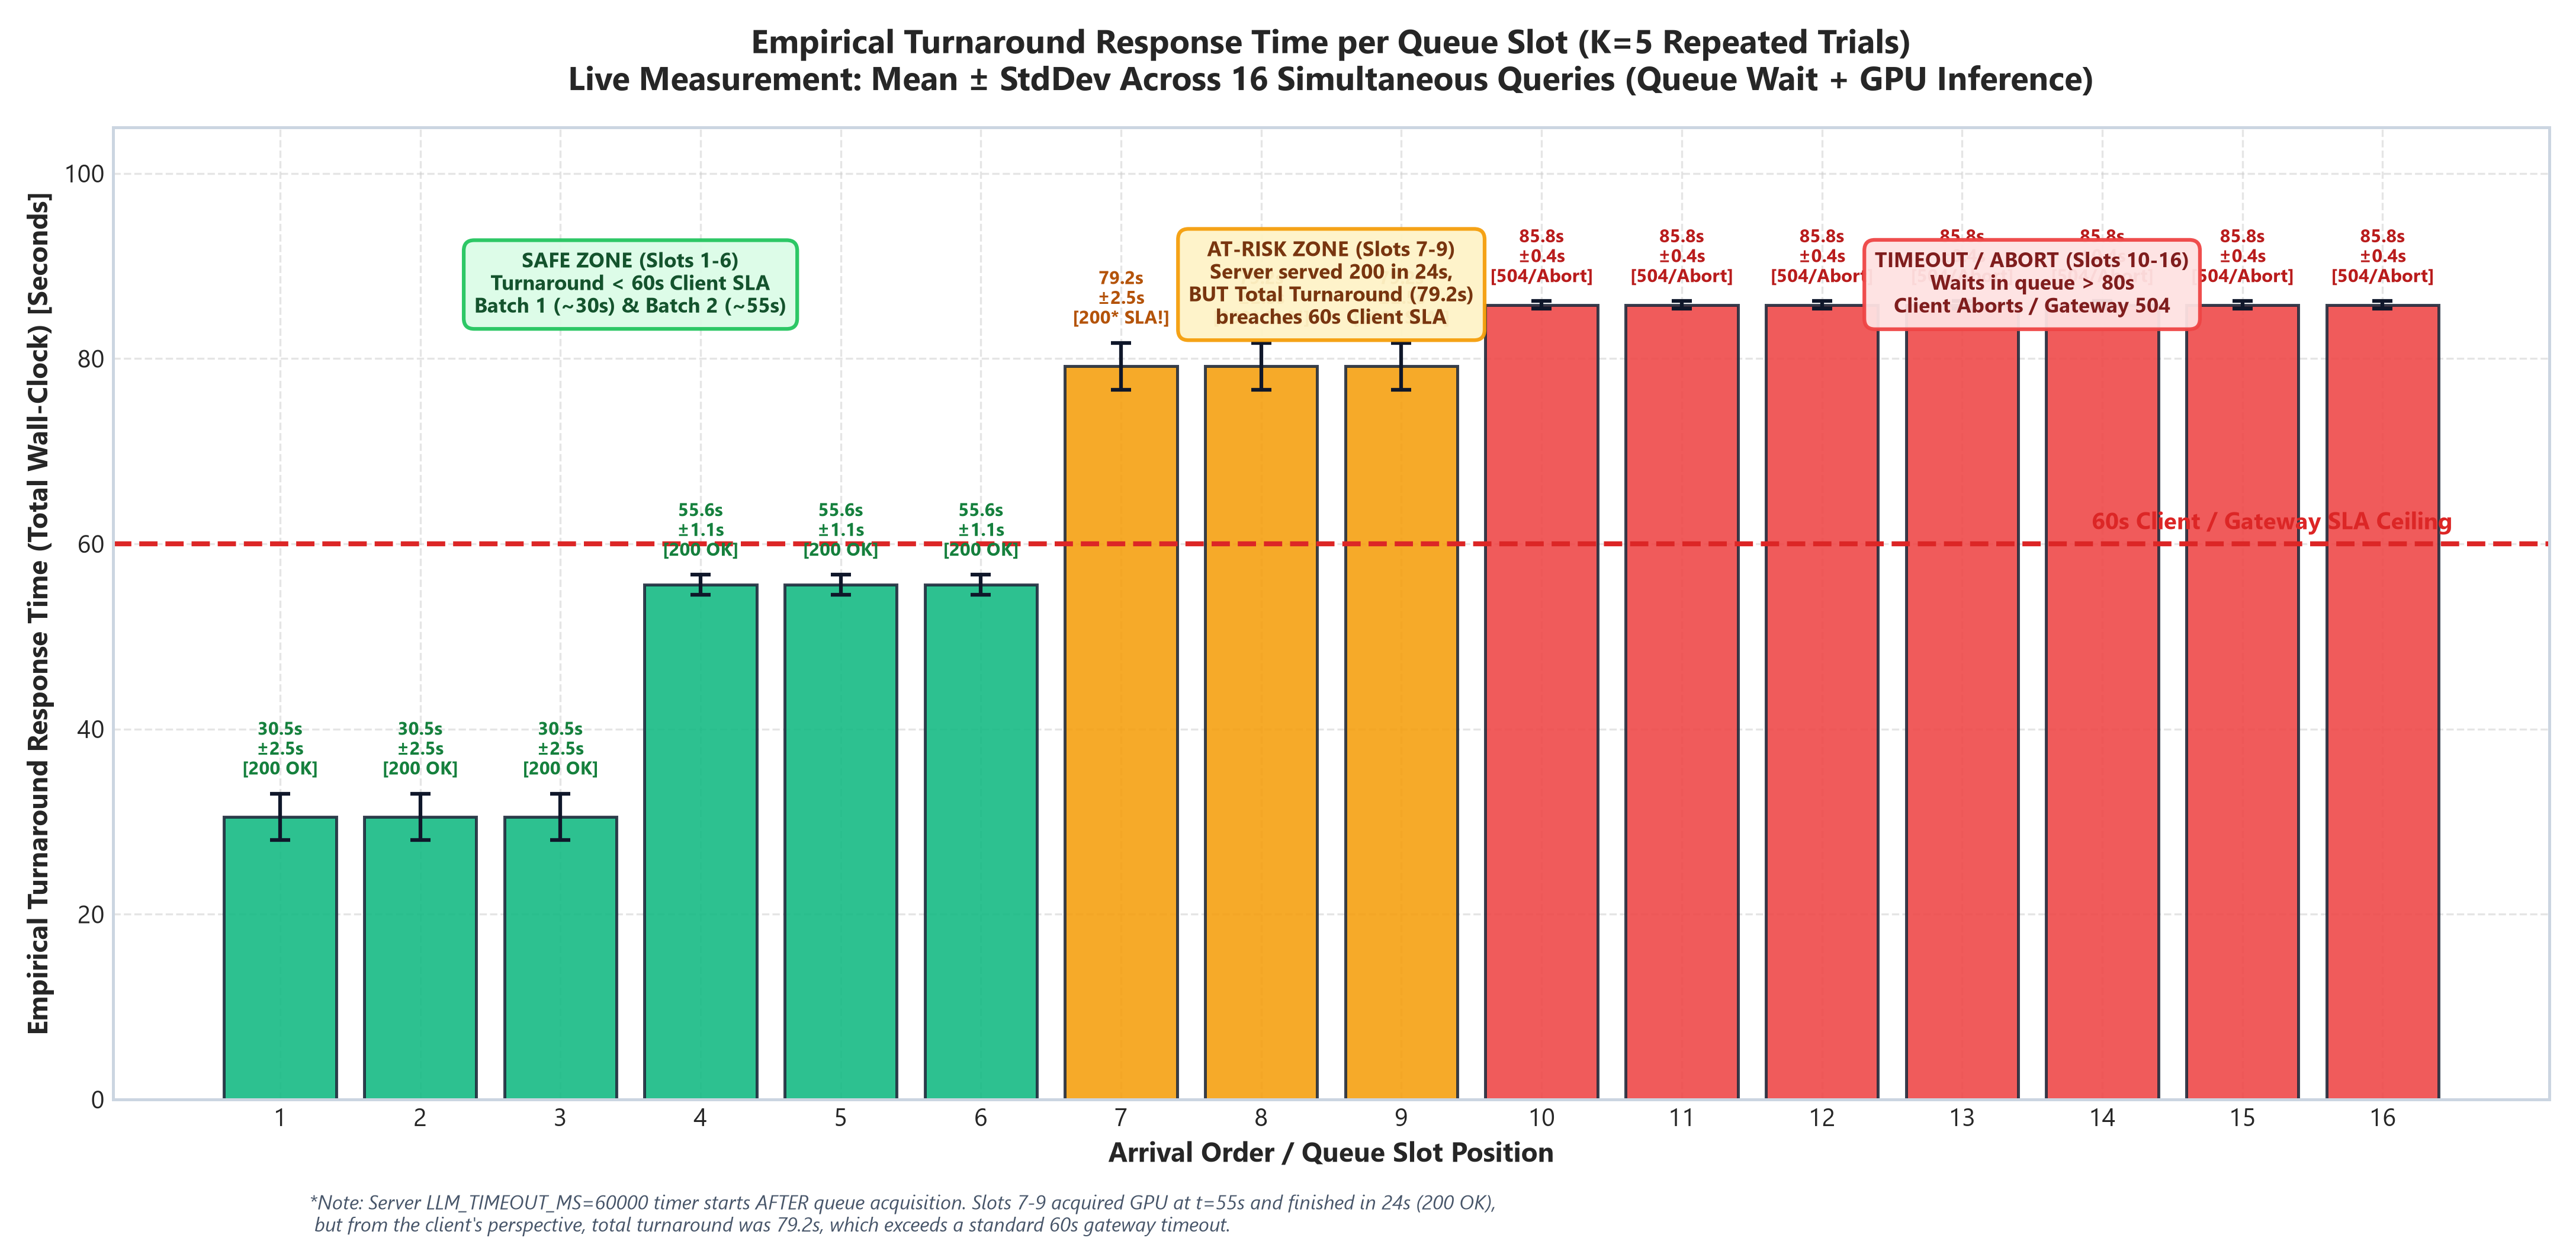
\includegraphics[width=0.92\textwidth]{assets/diagrams/empirical_k_fold_burst_turnaround.png}
\caption{Phân bố thời gian quay vòng theo nhóm 3~slot trong đợt dồn tải 16~yêu cầu lặp 5~lần (\textit{k-fold})}
\label{fig:thoi-gian-quay-vong-slot}
\end{figure}

Bảng~\ref{tab:thoi-gian-nhom-slot} và Hình~\ref{fig:thoi-gian-quay-vong-slot} cho thấy các yêu cầu trong cùng một đợt 3~slot hoàn thành gần như đồng thời theo từng bậc thời gian (khoảng 30,5~giây, 55,6~giây và 79,2~giây) thay vì xếp bậc đơn lẻ, chứng minh khả năng thực thi theo lô của GPU trong cấu hình thử nghiệm 3~slot cũng như lý do cấu hình mặc định cần giữ \texttt{LLM\_\allowbreak{}CONCURRENCY = 1} và từ chối nhanh ở chỗ thứ 9 để tránh tích tụ trễ quá hạn trên 85~giây.

\subsection{Đo trần thông lượng bền vững bằng phương pháp quét nhị phân}
\label{subsec:quet-nhi-phan}

Để tìm trần thông lượng bền vững cho từng kịch bản nghiệp vụ riêng lẻ làm cơ sở cho Bảng~\ref{tab:tran-thong-luong-kich-ban} (Chương~\ref{chap:ket-luan}), hệ thống áp dụng thuật toán \textbf{quét nhị phân qua ba hiệp liên tiếp}:

\begin{enumerate}
\item \textbf{Hiệp thô (bước tăng gấp đôi)}: Tăng dần tần suất đến hoặc số người dùng ảo theo cấp số nhân (\texttt{10 -> 40 -> 80 -> 160} hoặc \texttt{50 -> 100 -> 200 -> 400 -> 800}) cho tới khi vi phạm một trong ba ngưỡng Quy tắc~L1.
\item \textbf{Hiệp tinh chỉnh nhị phân}: Khoanh vùng biên giữa mức đạt cao nhất và mức vừa gãy để tìm ngưỡng giới hạn trên.
\item \textbf{Hiệp giữ tải chứng nhận 180~giây}: Khoá mức tải vừa xác định và chạy giữ tải liên tục ba phút qua ba lần đo để xác nhận tính bền vững (0,00\% lỗi và \texttt{p95}, \texttt{p99} dưới ngưỡng).
\end{enumerate}

Bảng~\ref{tab:ket-qua-quet-nhi-phan} tổng hợp đầy đủ các điểm đo trong quá trình quét và giữ tải của bốn kịch bản nghiệp vụ.

\begingroup\footnotesize
\setlength{\tabcolsep}{4pt}
\begin{longtable}{
  @{}>{\raggedright\arraybackslash}p{4.8cm}
  >{\raggedright\arraybackslash}p{1.8cm}
  >{\raggedleft\arraybackslash}p{1.5cm}
  >{\raggedleft\arraybackslash}p{1.6cm}
  >{\raggedleft\arraybackslash}p{1.7cm}
  >{\raggedleft\arraybackslash}p{1.2cm}
  >{\raggedright\arraybackslash}p{1.7cm}@{}
}
\caption{Kết quả quét nhị phân tìm trần thông lượng theo kịch bản nghiệp vụ}
\label{tab:ket-qua-quet-nhi-phan} \\
\toprule
\textbf{Kịch bản} & \textbf{Mức tải} & \texttt{p50} & \texttt{p95} & \texttt{p99} & \textbf{Lỗi} & \textbf{Kết luận} \\
\midrule
\endfirsthead
\caption[]{Kết quả quét nhị phân tìm trần thông lượng theo kịch bản nghiệp vụ (tiếp theo)} \\
\toprule
\textbf{Kịch bản} & \textbf{Mức tải} & \texttt{p50} & \texttt{p95} & \texttt{p99} & \textbf{Lỗi} & \textbf{Kết luận} \\
\midrule
\endhead
\midrule
\multicolumn{7}{r}{\textit{Xem tiếp ở trang sau}} \\
\endfoot
\bottomrule
\endlastfoot
Thao tác phiên trò chuyện (tải mở) & 50~RPS & 2,22~ms & 4,79~ms & 6,80~ms & 0,00\% & Đạt \\
Thao tác phiên trò chuyện (tải mở) & 100~RPS & 3,60~ms & 8,85~ms & 17,69~ms & 0,00\% & Đạt \\
Thao tác phiên trò chuyện (tải mở) & 200~RPS & 1,88~ms & 6,72~ms & 13,31~ms & 0,00\% & Đạt \\
Thao tác phiên trò chuyện (tải mở) & 400~RPS & 1,17~ms & 15,69~ms & 92,09~ms & 0,00\% & Đạt \\
Thao tác phiên trò chuyện (tải mở) & 800~RPS & 1,16~ms & 780,82~ms & 2.505,40~ms & 0,00\% & Không đạt \\
Thao tác phiên trò chuyện (giữ tải 180s) & 400~RPS & 1,26~ms & 10,63~ms & 160,50~ms & 0,00\% & Đạt \\
\midrule
Hành trình người dùng (tải đóng) & 100~VU & 5,44~ms & 95,25~ms & 139,13~ms & 0,00\% & Đạt \\
Hành trình người dùng (tải đóng) & 400~VU & 3,18~ms & 140,59~ms & 218,96~ms & 0,00\% & Đạt \\
Hành trình người dùng (tải đóng) & 800~VU & 2,12~ms & 816,95~ms & 941,17~ms & 0,00\% & Không đạt \\
\midrule
Đọc bài báo cache lạnh (tải mở) & 10~RPS & 17,14~ms & 44,62~ms & 84,18~ms & 0,00\% & Đạt \\
Đọc bài báo cache lạnh (tải mở) & 40~RPS & 15,46~ms & 62,85~ms & 119,48~ms & 0,00\% & Đạt \\
Đọc bài báo cache lạnh (tải mở) & 80~RPS & 18,20~ms & 55,85~ms & 75,03~ms & 0,00\% & Đạt \\
Đọc bài báo cache lạnh (tải mở) & 160~RPS & 44,08~ms & 64,34~ms & 251,29~ms & 0,00\% & Đạt \\
Đọc bài báo cache lạnh (giữ tải 180s) & 160~RPS & 43,34~ms & 51,92~ms & 178,97~ms & 0,00\% & Đạt \\
\midrule
Băm mật khẩu và xoay token (tải mở) & 4~RPS & 46,14~ms & 60,46~ms & 71,61~ms & 0,00\% & Đạt \\
Băm mật khẩu và xoay token (tải mở) & 8~RPS & 38,34~ms & 45,60~ms & 59,16~ms & 0,00\% & Đạt \\
Băm mật khẩu và xoay token (tải mở) & 16~RPS & 30,43~ms & 39,44~ms & 105,03~ms & 0,00\% & Đạt \\
Băm mật khẩu và xoay token (tải mở) & 32~RPS & 30,37~ms & 57,01~ms & 74,12~ms & 0,00\% & Đạt \\
Băm mật khẩu và xoay token (giữ tải 180s) & 32~RPS & 29,01~ms & 47,20~ms & 63,49~ms & 0,00\% & Đạt \\
\end{longtable}
\endgroup

Bảng~\ref{tab:ket-qua-quet-nhi-phan} định vị rõ điểm gãy của từng nhóm nghiệp vụ: kịch bản \texttt{CRUD} giữ ổn định \texttt{p95} dưới 16~ms từ 50 đến 400~RPS (giữ tải 180~giây đạt \texttt{p95} 10,63~ms) rồi vọt lên \texttt{p95} 780,82~ms và \texttt{p99} 2.505,40~ms kèm 857~yêu cầu bị loại bởi cơ chế tải mở của \texttt{k6} tại mức 800~RPS. Tương tự, hành trình người dùng chứng nhận tại 400~VU (trước khi vượt ngưỡng ở 800~VU), đọc bài báo với cache lạnh đạt trần 160~RPS (\texttt{p95} 51,92~ms), và nhóm băm mật khẩu kết hợp xoay vòng token đạt trần 32~RPS (\texttt{p95} 47,20~ms).

\subsection{Giám sát tài nguyên hệ thống khi chạy tải}
\label{subsec:telemetry-tai-nguyen}

Script thu thập \texttt{telemetry} lấy mẫu mỗi hai giây chỉ số CPU (tính theo phần trăm tương đương một lõi và phần trăm toàn máy), bộ nhớ làm việc của tiến trình Node.js và tiến trình \texttt{cloudflared} trong suốt đợt giữ tải. Bảng~\ref{tab:telemetry-tai-nguyen-ch6} tóm tắt hồ sơ tài nguyên theo từng đợt đo tải chính.

\begin{table}[htbp]
\centering
\caption{Chỉ số telemetry tài nguyên của tiến trình Node.js theo đợt đo tải}
\label{tab:telemetry-tai-nguyen-ch6}
\footnotesize
\setlength{\tabcolsep}{4pt}
\begin{tabularx}{\textwidth}{
  >{\raggedright\arraybackslash}X
  >{\raggedleft\arraybackslash}p{1.9cm}
  >{\raggedleft\arraybackslash}p{1.8cm}
  >{\raggedleft\arraybackslash}p{2.0cm}
  >{\raggedleft\arraybackslash}p{2.0cm}
  >{\raggedleft\arraybackslash}p{2.0cm}
}
\toprule
\textbf{Đợt đo tải} & \textbf{CPU tối đa (1 lõi)} & \textbf{CPU TB} & \textbf{CPU toàn máy tối đa} & \textbf{RAM thấp nhất} & \textbf{RAM cao nhất} \\
\midrule
Giữ tải chứng nhận 250~RPS & 88,50\% & 64,68\% & 5,50\% & 2.281,50~MB & 3.414,20~MB \\
Tải mật mã, cấu hình gốc & 310,20\% & 197,13\% & 19,40\% & 2.056,20~MB & 2.352,40~MB \\
Tải mật mã, sau tinh chỉnh nhóm luồng & 870,30\% & 189,38\% & 54,40\% & 2.264,30~MB & 4.386,30~MB \\
\bottomrule
\end{tabularx}
\end{table}

Đối chiếu hai dòng cuối của Bảng~\ref{tab:telemetry-tai-nguyen-ch6} cho thấy bằng chứng phần cứng trực tiếp của việc cấu hình nhóm luồng thực thi: mức CPU tối đa tương đương một lõi tăng từ 310,20\% lên 870,30\% (huy động đồng thời nhiều lõi CPU hơn cho tác vụ Argon2id khi có đợt dồn tải) trong khi mức CPU trung bình toàn đợt thậm chí giảm nhẹ (197,13\% xuống 189,38\%). Nhờ tận dụng tối đa khả năng xử lý song song trên đa lõi, các yêu cầu nhẹ không băm mật khẩu thoát nhanh khỏi nghẽn hàng đợi, khớp với mức giảm độ trễ 96,00\% ở Bảng~\ref{tab:tac-dong-thread-pool}.

\section{Kiểm thử bảo mật}
\label{sec:security-testing}

Thay vì dừng ở việc rà soát danh mục lỗi thụ động, kiểm thử bảo mật tập trung xác minh thực nghiệm toàn bộ các bất biến an toàn đã thiết kế ở Mục~\ref{subsec:bao-mat} và Chương~\ref{chap:thiet-ke-kien-truc}. Mỗi cơ chế bảo vệ được gắn với một phép thử quan sát được hành vi phản hồi theo phân loại OWASP Top~10 (Bảng~\ref{tab:anh-xa-bao-mat-owasp}).

\begin{table}[htbp]
\centering
\caption{Ánh xạ giữa hướng tấn công, cơ chế bảo mật và kết quả kiểm chứng}
\label{tab:anh-xa-bao-mat-owasp}
\footnotesize
\setlength{\tabcolsep}{4pt}
\begin{tabularx}{\textwidth}{
  >{\raggedright\arraybackslash}p{3.4cm}
  >{\raggedright\arraybackslash}p{4.3cm}
  >{\raggedright\arraybackslash}X
  >{\raggedright\arraybackslash}p{1.4cm}
}
\toprule
\textbf{Hướng tấn công (OWASP)} & \textbf{Cơ chế bảo mật} & \textbf{Phép thử kiểm chứng} & \textbf{Kết quả} \\
\midrule
Dò đoán mật khẩu (\texttt{A07}) & Băm mật khẩu bằng Argon2id, tham số \texttt{memory-hard} & Xác nhận CSDL chỉ lưu chuỗi băm \texttt{\$argon2id\$}, không lưu văn bản gốc & Đạt \\
\midrule
Tái sử dụng hoặc đánh cắp token (\texttt{A07}) & Xoay vòng refresh token một lần theo họ token (\texttt{token family}) & Dùng lại token đã xoay vòng lập tức thu hồi toàn bộ họ token & Đạt \\
\midrule
Chiếm quyền qua phiên bản token cũ (\texttt{A07}) & JWT mang \texttt{token\_version}, kiểm tra đối chiếu khi xác thực & Token cấp trước thời điểm đổi vai trò hoặc khoá tài khoản bị từ chối ngay & Đạt \\
\midrule
Tiêm mã SQL/NoSQL (\texttt{A03}) & \texttt{ValidationPipe} với \texttt{DTO} chặt chẽ, chuẩn hoá kiểu dữ liệu & Tải trọng đối tượng truy vấn lồng nhau trong bộ lọc bị chặn ở biên \texttt{DTO} & Đạt \\
\midrule
Tấn công vét cạn và làm ngập API (\texttt{A04}) & Giới hạn tần suất (\texttt{rate limiting}) phân tầng theo nhóm endpoint & Sau năm lần đăng nhập sai trong một phút trả về mã \texttt{429} & Đạt \\
\midrule
Làm cạn kiệt tài nguyên suy luận (\texttt{A04}) & Hàng đợi \texttt{LlmQueue} giới hạn tối đa và từ chối nhanh \texttt{429} & Khi chạm ngưỡng 8~chỗ chờ trả về \texttt{429}, không gây treo tiến trình & Đạt \\
\midrule
Leo thang đặc quyền (\texttt{A01}) & Bảo vệ đa lớp (\texttt{JwtAuthGuard}, \texttt{RolesGuard}, kiểm tra service) & Token vai trò người dùng thường gọi route quản trị trả về \texttt{403} & Đạt \\
\midrule
Dò lộ định danh tài nguyên (\texttt{A01}) & Ràng buộc sở hữu theo \texttt{user\_id} trên mọi truy vấn phiên & Truy cập phiên của người dùng khác trả về \texttt{404} thay vì \texttt{403} & Đạt \\
\midrule
Tiêm thực thể XML ngoài (\texttt{XXE}, \texttt{A05}) & Chặn khai báo \texttt{DOCTYPE} và \texttt{ENTITY} trong XML đầu vào & Gói tin XML chứa \texttt{DOCTYPE} bị từ chối với mã \texttt{400} & Đạt \\
\midrule
Từ chối dịch vụ bằng regex (\texttt{ReDoS}, \texttt{A03}) & Thoát ký tự đặc biệt trước khi biên dịch regex tìm kiếm & Chuỗi chứa ký tự đặc biệt regex được đối chiếu theo nghĩa đen an toàn & Đạt \\
\midrule
Sửa hoặc xoá dấu vết kiểm toán (\texttt{A01}) & Tập hợp \texttt{admin\_audit\_logs} chỉ cho phép ghi thêm (\texttt{append-only}) & Không tồn tại endpoint hoặc phương thức sửa, xoá nhật ký kiểm toán & Đạt \\
\bottomrule
\end{tabularx}
\end{table}

Bảng~\ref{tab:gioi-han-tan-suat-ch6} tổng hợp cấu hình giới hạn tần suất theo từng nhóm route nhằm phòng chống vét cạn và cạn kiệt tài nguyên (kế thừa và bổ sung hạng mục đọc hàng loạt bài báo cho danh mục tại Mục~\ref{subsec:bao-mat}, Chương~\ref{chap:phan-tich-yeu-cau}).

\begin{table}[htbp]
\centering
\caption{Cấu hình giới hạn tần suất theo từng nhóm route}
\label{tab:gioi-han-tan-suat-ch6}
\small
\begin{tabularx}{\textwidth}{
  >{\raggedright\arraybackslash}p{4.3cm}
  >{\raggedleft\arraybackslash}p{1.8cm}
  >{\raggedleft\arraybackslash}p{1.8cm}
  >{\raggedright\arraybackslash}X
}
\toprule
\textbf{Nhóm route} & \textbf{Hạn mức} & \textbf{Chu kỳ} & \textbf{Cơ sở thiết lập} \\
\midrule
Đăng ký tài khoản & 5 & 60~giây & Ngăn tạo hàng loạt tài khoản và tiêu hao CPU qua Argon2id \\
Đăng nhập & 10 & 60~giây & Chặn tấn công dò mật khẩu tự động \\
Xoay vòng token & 30 & 60~giây & Cho phép làm mới phiên hợp lệ nhưng giới hạn lạm dụng \\
Đổi mật khẩu & 5 & 60~giây & Giới hạn tần suất thao tác mật mã nhạy cảm \\
Hỏi đáp RAG (đã đăng nhập) & 20 & 60~giây & Bảo vệ hàng đợi suy luận GPU có số luồng hạn chế \\
Hỏi đáp RAG (khách vãng lai) & 10 & 60~giây & Hạn mức chặt hơn cho truy cập không định danh \\
Đọc hàng loạt bài báo (\texttt{papers}) & 30 & 60~giây & Mỗi lần gọi có thể đọc tối đa 20~bài báo từ kho \\
Mặc định toàn cục & 120 & 60~giây & Ngưỡng nền bảo vệ toàn bộ các endpoint còn lại \\
\bottomrule
\end{tabularx}
\end{table}

Bảng~\ref{tab:tham-so-argon2id-ch6} liệt kê các tham số mật mã của Argon2id được kiểm chứng cố định trong mã nguồn. Ba tham số đầu (\texttt{memoryCost}, \texttt{timeCost}, \texttt{parallelism}) quyết định trực tiếp độ kháng tấn công bằng GPU/ASIC và tuyệt đối không được hạ thấp; thời gian giới hạn trên (5,01~giây) dùng để kiểm soát tải tính toán và ngăn tự gây nghẽn dịch vụ.

\begin{table}[htbp]
\centering
\caption{Tham số thuật toán băm mật khẩu Argon2id}
\label{tab:tham-so-argon2id-ch6}
\small
\begin{tabularx}{\textwidth}{
  >{\raggedright\arraybackslash}p{4.6cm}
  >{\raggedright\arraybackslash}p{3.4cm}
  >{\raggedright\arraybackslash}X
}
\toprule
\textbf{Tham số} & \textbf{Giá trị} & \textbf{Vai trò bảo mật} \\
\midrule
Biến thể thuật toán & \texttt{Argon2id} & Kết hợp ưu thế kháng tấn công GPU (\texttt{Argon2d}) và kênh bên (\texttt{Argon2i}) \\
\midrule
Chi phí bộ nhớ (\texttt{memoryCost}) & 65.536~KiB (64~MiB) & Tạo áp lực bộ nhớ lớn nhằm vô hiệu hoá dò tìm song song trên GPU \\
\midrule
Số vòng lặp (\texttt{timeCost}) & 3 & Tăng chi phí thời gian cho mỗi lần thử mật khẩu \\
\midrule
Mức song song (\texttt{parallelism}) & 4 & Khớp với cấu hình 4~luồng thực thi của Node.js \\
\midrule
Thời gian tính toán tối đa & 5,01~giây & Chặn nguy cơ treo tiến trình khi phát sinh nhiều lượt băm \\
\bottomrule
\end{tabularx}
\end{table}

Bảng~\ref{tab:phep-thu-bao-mat-ch6} tổng hợp toàn bộ 15~phép thử nghiệm thu bảo mật đã thực thi tự động và đầu cuối.

\begingroup\small
\setlength{\tabcolsep}{5pt}
\begin{longtable}{
  @{}>{\raggedright\arraybackslash}p{4.6cm}
  >{\raggedright\arraybackslash}p{2.9cm}
  >{\raggedright\arraybackslash}p{1.6cm}
  >{\raggedright\arraybackslash}p{5.5cm}@{}
}
\caption{Danh mục 15~phép thử kiểm chứng bất biến bảo mật}
\label{tab:phep-thu-bao-mat-ch6} \\
\toprule
\textbf{Phép thử nghiệm thu} & \textbf{Nhóm kiểm thử} & \textbf{Kết quả} & \textbf{Minh chứng quan sát} \\
\midrule
\endfirsthead
\caption[]{Danh mục 15~phép thử kiểm chứng bất biến bảo mật (tiếp theo)} \\
\toprule
\textbf{Phép thử nghiệm thu} & \textbf{Nhóm kiểm thử} & \textbf{Kết quả} & \textbf{Minh chứng quan sát} \\
\midrule
\endhead
\midrule
\multicolumn{4}{r}{\textit{Xem tiếp ở trang sau}} \\
\endfoot
\bottomrule
\endlastfoot
Chỉ lưu chuỗi băm, không lưu mật khẩu thô & Xác thực & Đạt & Bản ghi người dùng lưu tiền tố \texttt{\$argon2id\$} \\
Năm lần đăng nhập thất bại liên tiếp & Chống vét cạn & Đạt & Lần thử kế tiếp trả về HTTP~\texttt{429} \\
Dùng lại refresh token cũ đã xoay vòng & Xác thực & Đạt & Toàn bộ họ token liên quan bị thu hồi \\
Hai yêu cầu xoay vòng token đồng thời & Xác thực & Đạt & Chỉ một yêu cầu thành công, yêu cầu trùng bị chặn \\
Dùng JWT cấp trước khi đổi vai trò & Phân quyền & Đạt & \texttt{token\_version} lệch làm token cũ mất hiệu lực \\
Dùng JWT đã hết hạn & Xác thực & Đạt & Trả về HTTP~\texttt{401} \\
Truy cập phiên của người dùng khác & Sở hữu dữ liệu & Đạt & Trả về HTTP~\texttt{404} (tránh lộ sự tồn tại) \\
Truy cập phiên đã đánh dấu xoá mềm & Sở hữu dữ liệu & Đạt & Trả về HTTP~\texttt{404} \\
Truyền đối tượng NoSQL injection & Kiểm tra đầu vào & Đạt & Bị từ chối tại \texttt{ValidationPipe} với HTTP~\texttt{400} \\
Chuỗi tìm kiếm có ký tự đặc biệt regex & Chống \texttt{ReDoS} & Đạt & Ký tự đặc biệt được thoát và khớp theo nghĩa đen \\
Gửi XML chứa khai báo \texttt{DOCTYPE} & Chống \texttt{XXE} & Đạt & Bị từ chối ngay tại bộ phân tích XML với HTTP~\texttt{400} \\
Người dùng thường gọi route quản trị & Phân quyền & Đạt & Trả về HTTP~\texttt{403} \\
Quản trị viên tự khoá hoặc xoá vai trò cuối & Phân quyền & Đạt & Từ chối thao tác với HTTP~\texttt{400} \\
Vô hiệu hoá tài khoản đang hoạt động & Phân quyền & Đạt & Toàn bộ access và refresh token bị thu hồi tức thời \\
Nhật ký kiểm toán chỉ cho phép ghi thêm & Toàn vẹn dấu vết & Đạt & Không tồn tại API sửa hoặc xoá bản ghi kiểm toán \\
\end{longtable}
\endgroup

\section{Đánh giá tài nguyên}
\label{sec:danh-gia-tai-nguyen-chi-phi}

Đánh giá tài nguyên hệ thống được thực hiện trên hai trục: hồ sơ bộ nhớ (\texttt{RSS}) của tiến trình máy chủ ứng dụng và hiệu năng kết xuất phía thiết bị người dùng, kèm tổng hợp thông số tài nguyên phần cứng của hạ tầng suy luận cục bộ trên máy trạm GPU. Về mặt giám sát số liệu, trong giai đoạn đánh giá, backend đã mở điểm thu thập chỉ số \textbf{Prometheus cục bộ} ghi nhận chuỗi thời gian bộ nhớ \texttt{RSS} và histogram độ trễ phục vụ kiểm chứng (trong khi việc hoàn thiện ngăn xếp quan trắc tập trung hoàn chỉnh với bảng điều khiển Grafana, Grafana Loki và OpenTelemetry cho môi trường production được ghi nhận ở Chương~\ref{chap:ket-luan}).

Bảng~\ref{tab:ho-so-rss-ch6} tổng hợp hồ sơ bộ nhớ \texttt{RSS} của tiến trình máy chủ thu thập qua hai cửa sổ quan sát sáng và tối trong ngày 08/11/2026 với tổng cộng 441~mẫu từ Prometheus cục bộ.

\begin{table}[htbp]
\centering
\caption{Hồ sơ bộ nhớ (\texttt{RSS}) của tiến trình máy chủ theo chu kỳ hoạt động (441~mẫu)}
\label{tab:ho-so-rss-ch6}
\small
\begin{tabularx}{\textwidth}{
  >{\raggedright\arraybackslash}p{4.4cm}
  >{\raggedright\arraybackslash}p{4.3cm}
  >{\raggedright\arraybackslash}X
}
\toprule
\textbf{Trạng thái hệ thống} & \textbf{Khoảng giá trị đo được} & \textbf{Đặc trưng vận hành} \\
\midrule
Nhàn rỗi, không có luồng suy luận (377/441 mẫu) & Trung bình 89,81~MiB (42,6--415,0~MiB) & Chiếm 85,5\% thời gian quan sát; chỉ giữ heap JavaScript và kết nối nền \\
\midrule
Hoạt động suy luận, tải chuẩn (nhóm 64 mẫu) & Trung bình 1,46~GiB (mức ổn định 1,45~GiB) & Phục vụ luồng sinh văn bản \texttt{SSE} đang mở ngữ cảnh \\
\midrule
Hoạt động suy luận, thử nghiệm 3~luồng song song & 2,09~GiB & Mức đỉnh khi chạy đồng thời 3~slot suy luận thử nghiệm \\
\midrule
Khởi động lại và nạp mô hình vào bộ nhớ & 2,83~GiB & Đỉnh cao nhất trong toàn bộ 441~mẫu khi tải trọng số \\
\midrule
Kết thúc chu kỳ, đã giải phóng tài nguyên & 58,5~MiB đến 65,7~MiB & Trở về thấp hơn đường nền, chứng minh không rò rỉ bộ nhớ \\
\bottomrule
\end{tabularx}
\end{table}

Phân bố hai nhóm rời rạc quanh ngưỡng 500~MiB trong Bảng~\ref{tab:ho-so-rss-ch6} (khoảng cách gần hai bậc độ lớn giữa đường nền 89,81~MiB và trạng thái suy luận 1,46~GiB) xác nhận bộ nhớ tăng vọt có chu kỳ theo vòng đời cấp phát C++ cho ma trận và ngữ cảnh LLM rồi giải phóng triệt để khi luồng \texttt{SSE} kết thúc, hoàn toàn không có xu hướng rò rỉ tích luỹ theo thời gian (JavaScript heap duy trì ổn định trong khoảng 45--60~MiB).

Ở phía trình duyệt người dùng, Bảng~\ref{tab:web-vitals-lighthouse-ch6} và Hình~\ref{fig:ket-qua-lighthouse} trình bày kết quả kiểm toán Web Vitals bằng Lighthouse trên bản dựng production sau khi áp dụng các tối ưu ở Chương~\ref{chap:thiet-ke-kien-truc} (tải trì hoãn thư viện KaTeX, giới hạn tỉ lệ điểm ảnh WebGL ở 1,15 và gom đệm token \texttt{SSE} theo chu kỳ 30~ms).

\begin{table}[htbp]
\centering
\caption{Chỉ số Web Vitals đo bằng Lighthouse trên bản dựng production}
\label{tab:web-vitals-lighthouse-ch6}
\small
\begin{tabularx}{\textwidth}{
  >{\raggedright\arraybackslash}X
  >{\raggedleft\arraybackslash}p{2.6cm}
  >{\raggedleft\arraybackslash}p{2.6cm}
  >{\raggedright\arraybackslash}p{2.0cm}
}
\toprule
\textbf{Chỉ số Lighthouse / Web Vitals} & \textbf{Giá trị đo được} & \textbf{Ngưỡng chuẩn} & \textbf{Kết luận} \\
\midrule
Điểm hiệu năng (\textit{Performance}) & 97 / 100 & $\ge$ 90 & Đạt \\
Khả năng tiếp cận (\textit{Accessibility}) & 100 / 100 & 100 & Đạt \\
Thực hành tốt nhất (\textit{Best Practices}) & 100 / 100 & 100 & Đạt \\
Hiển thị nội dung đầu tiên (\texttt{FCP}) & 0,9~s & $\le$ 1,8~s & Đạt \\
Hiển thị nội dung lớn nhất (\texttt{LCP}) & 1,0~s & $\le$ 2,5~s & Đạt \\
Tổng thời gian chặn luồng chính (\texttt{TBT}) & 40~ms & $\le$ 200~ms & Đạt \\
Độ lệch bố cục tích luỹ (\texttt{CLS}) & 0,002 & $\le$ 0,1 & Đạt \\
\bottomrule
\end{tabularx}
\end{table}

\begin{figure}[htbp]
\centering
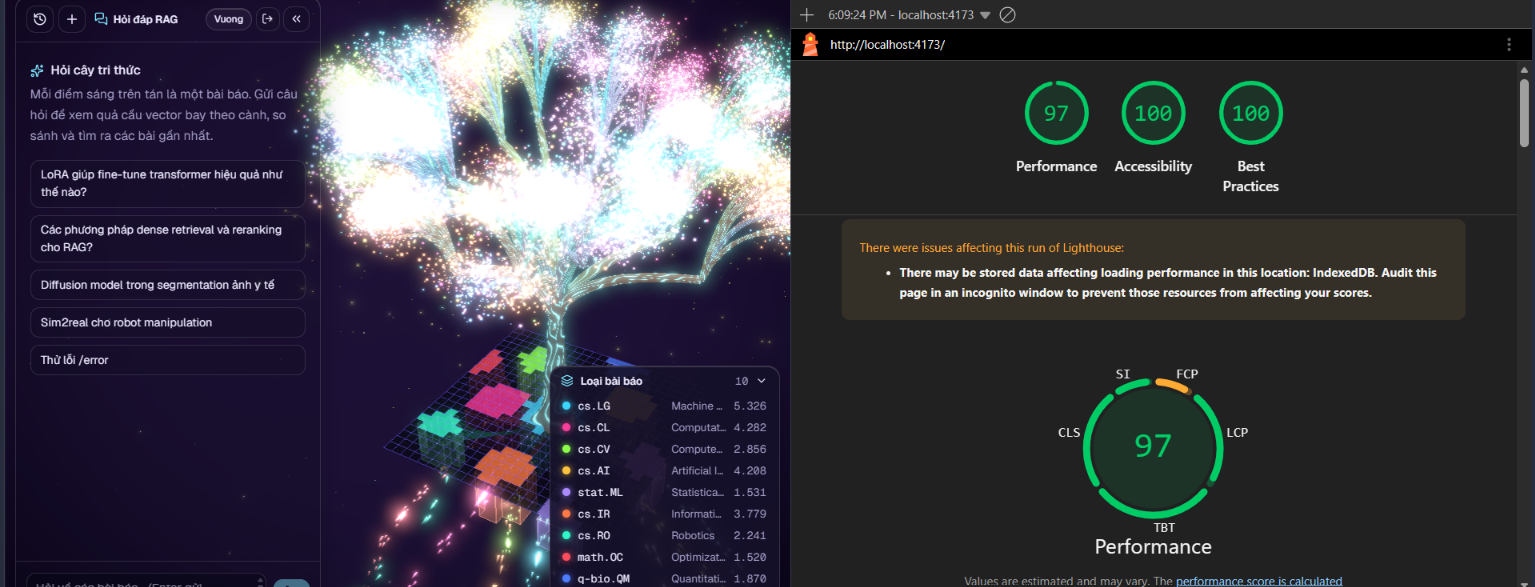
\includegraphics[width=0.92\textwidth]{assets/screenshots/lighthouse_audit.png}
\caption{Kết quả kiểm toán hiệu năng, khả năng tiếp cận và Web Vitals bằng Lighthouse trên bản dựng production}
\label{fig:ket-qua-lighthouse}
\end{figure}

Song song với Lighthouse, Bảng~\ref{tab:toi-uu-3d-dda-ch6} đo lường trực tiếp hiệu quả tối ưu không gian 3D bằng thuật toán duyệt lưới \texttt{3D DDA} trên tập lưới không gian phục vụ chiếu tia chọn điểm (\texttt{raycasting}) so với phương pháp quét tuyến tính ban đầu.

\begin{table}[htbp]
\centering
\caption{Tác động tối ưu chiếu tia không gian 3D bằng lưới duyệt 3D DDA}
\label{tab:toi-uu-3d-dda-ch6}
\small
\begin{tabularx}{\textwidth}{
  >{\raggedright\arraybackslash}X
  >{\raggedleft\arraybackslash}p{2.6cm}
  >{\raggedleft\arraybackslash}p{2.9cm}
  >{\raggedright\arraybackslash}p{3.6cm}
}
\toprule
\textbf{Tác vụ tương tác 3D} & \textbf{Phương pháp cũ} & \textbf{Thuật toán 3D DDA} & \textbf{Hệ số tăng tốc} \\
\midrule
Chiếu một tia chọn điểm (\texttt{raycasting}) & 1,20~ms & 0,022~ms & Nhanh hơn 56 lần \\
Chuyển đổi bộ lọc nhánh tri thức & 2,31~ms & 0,27~ms & Nhanh hơn 8,6 lần \\
Một bước tính toán chuyển động & 0,65~ms & 0,0002~ms & Nhanh hơn khoảng 2.600 lần \\
\bottomrule
\end{tabularx}
\end{table}

Thử nghiệm đối chiếu trên 40~tia ngẫu nhiên xác nhận thuật toán \texttt{3D DDA} trả về tập điểm trúng trùng khớp 100\% với phương pháp quét cũ, đồng thời giảm thời gian kết xuất khung hình trung vị 57\% ở chế độ tối và 65\% ở chế độ sáng.

Về tài nguyên hạ tầng suy luận phục vụ đánh giá, Bảng~\ref{tab:cau-hinh-phan-cung-ai-ch6} tổng hợp cấu hình phần cứng thực tế và các giới hạn cấp phát sử dụng cho đợt đo.

\begin{table}[htbp]
\centering
\caption{Cấu hình phần cứng và tham số suy luận của đợt đánh giá}
\label{tab:cau-hinh-phan-cung-ai-ch6}
\small
\begin{tabularx}{\textwidth}{
  >{\raggedright\arraybackslash}p{3.2cm}
  >{\raggedright\arraybackslash}p{3.8cm}
  >{\raggedleft\arraybackslash}p{2.1cm}
  >{\raggedright\arraybackslash}X
}
\toprule
\textbf{Hạng mục} & \textbf{Thông số cấu hình} & \textbf{Giá trị} & \textbf{Vai trò trong đánh giá} \\
\midrule
Bộ xử lý đồ hoạ (GPU) & NVIDIA RTX~4060 & 8~GB VRAM & Thực thi mô hình sinh cục bộ trên CUDA \\
\midrule
Mô hình ngôn ngữ & \texttt{Qwen2.5-\allowbreak{}7B-\allowbreak{}Instruct} (\texttt{GGUF}, \texttt{Q4\_\allowbreak{}K\_\allowbreak{}M}) & 4,68~GB VRAM & Lưu trọn bộ trọng số lượng tử hoá trên VRAM \\
\midrule
Cửa sổ ngữ cảnh & Tối đa & 8.192~token & Giới hạn chiều dài ngữ cảnh cho mỗi lượt hỏi đáp \\
\midrule
Nhiệt độ suy luận & Tham số cố định lúc đo & 0 & Cố định \texttt{temperature = 0} để tái lập kết quả (vận hành mặc định dùng \texttt{0,2}) \\
\midrule
Hàng đợi mặc định & Chế độ chuẩn & 1~slot + 8~chờ & Điều tiết lưu lượng tránh tràn VRAM \\
\midrule
Thời hạn suy luận & Mức cấu hình ứng dụng & 60~giây & Ngăn treo luồng khi sinh câu trả lời quá dài \\
\bottomrule
\end{tabularx}
\end{table}

Bảng~\ref{tab:diem-nghen-ky-thuat-ch6} tổng hợp sáu hạn chế kỹ thuật quan sát được ngay trong pha đánh giá hiệu năng và vận hành của Chương~6, làm cơ sở kỹ thuật liên kết trực tiếp với danh mục mười hạn chế tổng hợp toàn hệ thống ở Mục~\ref{sec:han-che} (Chương~\ref{chap:ket-luan}).

\begin{table}[htbp]
\centering
\caption{Các điểm nghẽn kỹ thuật ghi nhận trong pha đánh giá hiệu năng}
\label{tab:diem-nghen-ky-thuat-ch6}
\footnotesize
\setlength{\tabcolsep}{4pt}
\begin{tabularx}{\textwidth}{
  >{\raggedright\arraybackslash}p{3.1cm}
  >{\raggedright\arraybackslash}p{4.2cm}
  >{\raggedright\arraybackslash}p{3.5cm}
  >{\raggedright\arraybackslash}X
}
\toprule
\textbf{Điểm nghẽn quan sát} & \textbf{Biểu hiện định lượng} & \textbf{Giảm thiểu hiện tại} & \textbf{Hướng khắc phục} \\
\midrule
Đơn luồng xử lý suy luận mặc định & Lượt hỏi đáp đầy đủ có \texttt{p50} 32,67~giây và \texttt{p95} 45,46~giây & Hàng đợi \texttt{LlmQueue} ưu tiên từ chối nhanh \texttt{429} & Nâng cấp runtime hỗ trợ \textit{continuous batching} hoặc thêm GPU \\
\midrule
Tăng độ trễ đọc khi cache lạnh ở tải cao & \texttt{p50} đọc bài báo cache lạnh tăng từ 18,20~ms lên 43,34~ms ở 160~RPS & Bộ nhớ đệm \texttt{LRUCache} gắn bộ đếm thế hệ & Tối ưu chỉ mục phân trang và thêm nhớ đệm phân tán \\
\midrule
Độ trễ ghi qua \texttt{tunnel} MongoDB & \texttt{p50} đổi tên phiên lên tới 193,40~ms (do \texttt{RTT} 114~ms) & Thực thi song song truy vấn độc lập & Giảm độ trễ mạng tới MongoDB hoặc triển khai nội vùng \\
\midrule
Sai lệch histogram toàn cục do gộp luồng \texttt{SSE} & \texttt{p95} bị ghim ở trần bucket 25--30~giây dù \texttt{p95} REST thuần là 41,96~ms & Tách riêng REST và \texttt{SSE} khi phân tích 132~mẫu & Tách hai bộ histogram độc lập cho REST và \texttt{SSE} theo \texttt{TTFT} \\
\midrule
Đỉnh bộ nhớ khi khởi động lại mô hình & Tiến trình chạm đỉnh 2,83~GiB khi nạp lại trọng số & Nạp nền bất đồng bộ, giữ \texttt{/health/live} & Nạp phân tầng và kiểm soát bộ nhớ đệm trang trọng số \\
\midrule
Giới hạn trên một nút GPU đơn lẻ & Không tự phân tải suy luận ngang qua nhiều máy chủ & Điều tiết lưu lượng bằng hàng đợi 8~chỗ chờ & Tách dịch vụ suy luận và cân bằng tải hàng đợi phân tán \\
\bottomrule
\end{tabularx}
\end{table}

Hiện tượng ghim trần histogram ở Bảng~\ref{tab:diem-nghen-ky-thuat-ch6} được kiểm chứng rõ trên 132~mẫu thu thập ở cửa sổ đo buổi tối: 64~mẫu REST thuần phân bố trong dải 4,75--242~ms (trung vị 41,96~ms ở phân vị 95), trong khi 68~mẫu có luồng \texttt{SSE} kéo dài thời gian đóng kết nối HTTP bị dồn vào đúng bucket cao nhất (25--30~giây) trong mảng \texttt{BUCKETS} của Prometheus cục bộ, tạo chênh lệch biểu kiến tới 669~lần dù bản chất là do gộp chung hai loại lưu lượng có bản chất thời gian khác nhau vào một metric.

Hình~\ref{fig:chuoi-bao-ve-suy-luan} tổng hợp chuỗi cơ chế bảo vệ của hạ tầng suy luận khi tải đồng thời chạm ngưỡng bão hoà.

\begin{figure}[htbp]
\centering
\resizebox{\textwidth}{!}{%
\begin{tikzpicture}[
    node distance=0.85cm and 1.25cm,
    boxnode/.style={ragbox, text width=3.3cm, minimum height=1.15cm, font=\footnotesize\sffamily}
]
    \node[boxnode] (req) {Yêu cầu hỏi đáp};
    \node[boxnode, right=of req, text width=3.6cm] (queue) {Hàng đợi \texttt{LlmQueue}\\1~slot + 8~chỗ chờ};
    \node[boxnode, below=1.1cm of queue, fill=orange!10, draw=orange!75!black] (ff) {Từ chối nhanh\\HTTP~\texttt{429} (\texttt{LLM\_QUEUE\_FULL})};
    \node[boxnode, right=1.35cm of queue, text width=3.5cm] (eng) {Suy luận cục bộ\\RTX~4060, \texttt{Qwen2.5-7B}};
    \node[ragdecision, right=1.35cm of eng, text width=2.4cm, font=\footnotesize\sffamily] (gate) {Cổng căn cứ\\$\ge 0{,}3$ (Top-3)?};
    \node[boxnode, right=1.45cm of gate, fill=primaryBlue!18] (out) {Phát trực tiếp qua \texttt{SSE}};
    \node[boxnode, below=1.1cm of gate, text width=3.5cm, fill=orange!8, draw=orange!75!black] (nc) {Thông báo từ chối\\thiếu căn cứ};

    \draw[ragarrow] (req) -- (queue);
    \draw[ragarrow] (queue) -- node[above, font=\scriptsize] {Còn chỗ} (eng);
    \draw[ragarrow] (queue) -- node[right, font=\scriptsize] {Hàng đầy} (ff);
    \draw[ragarrow] (eng) -- (gate);
    \draw[ragarrow] (gate) -- node[above, font=\scriptsize] {Đạt} (out);
    \draw[ragarrow] (gate) -- node[right, font=\scriptsize] {Không đạt} (nc);
\end{tikzpicture}%
}
\caption{Chuỗi cơ chế bảo vệ của hạ tầng suy luận khi tài nguyên bị bão hoà}
\label{fig:chuoi-bao-ve-suy-luan}
\end{figure}
